%	\parbox{\linewidth}{\centering\fontsize{18}{22}\selectfont\linespread{1}\selectfont\bfseries La répartition de l'hydrogène atomique (\HI) cinématiquement froid et chaud et son lien avec la formation stellaire dans les galaxies proches}
\documentclass[final,oneside]{StylesAndSettings/uqthesis} 
\usepackage[T1]{fontenc}
%\usepackage[french]{babel}
%\frenchsetup{SmallCapsFigTabCaptions=false}
%\addto\captionsfrench{\renewcommand{\tablename}{Tableau}}
\usepackage{caption}
\usepackage{adjustbox}
\usepackage{subcaption}
\usepackage{tabularx}
\usepackage{array}
\usepackage{xcolor}
\usepackage{bm}
\usepackage{pdfpages}
%\usepackage[none]{hyphenat} 

\renewcommand{\contentsname}{Table des matières} %for table of contents to be in french 
\renewcommand{\bibname}{Bibliographie}


\setlength{\footskip}{9mm}
\newcolumntype{L}[1]{>{\raggedright\arraybackslash}p{#1}}









\RequirePackage[authoryear,round]{natbib}
\usepackage{cite}				 
\usepackage{pdfpages}			 
\usepackage{wrapfig}			 
\usepackage{graphicx}
\usepackage{bm} 				 
\usepackage{upgreek}			 
\usepackage{dsfont}				 
\usepackage{simplewick}			 
\usepackage{mathtools}		     
\usepackage{framed}			     
\usepackage{microtype}			 
\usepackage{marvosym}			 
\usepackage{color}				 
\usepackage{transparent}	     
\usepackage{placeins}			 
\usepackage{mdframed,mdwlist}    
\usepackage{float}               
\usepackage{mathdots}            
\usepackage{eucal}               
\usepackage{array}               
\usepackage{stmaryrd}            
\usepackage{pifont}              
\usepackage{lipsum}              
\usepackage{enumerate}           
\usepackage[all]{xy}             
\usepackage[utf8]{inputenc}      
\usepackage{fancyhdr}            
\usepackage{blindtext}           
\usepackage{tikz}                
\usetikzlibrary{shapes.geometric, arrows}
\usepackage[figuresright]{rotating}	
\usepackage{chngcntr} 

\usepackage{ragged2e}
\AtBeginDocument{\justifying} 

\usepackage{caption} 
\usepackage{titlesec} 
\usepackage{multirow} 
\usepackage{indentfirst}
\geometry{left=2.5cm,right=1.5cm,top=2.5cm,bottom=2.5cm}  


\settrimmedsize{\stockheight}{\stockwidth}{*}
\settypeblocksize{\textheight}{\textwidth}{*}
\checkandfixthelayout
\setlength{\evensidemargin}{0pt}
\setlength{\oddsidemargin}{0pt}




\newcommand{\via}{\textit{via}} 
\newcommand{\ie}{\textit{i.e.}} 
\newcommand{\eg}{\textit{e.g.}} 
\newcommand{\etc}{\textit{etc.}} 
\newcommand{\vv}{\textit{vice versa}} 
\newcommand{\viz}{\textit{viz}.} 
\newcommand{\cf}{\textit{cf}.} 
\newcommand{\apr}{\textit{a priori}} 
\newcommand{\apo}{\textit{a posteriori}} 
\newcommand{\vivo}{\textit{in vivo}} 
\newcommand{\situ}{\textit{in situ}} 
\newcommand{\silico}{\textit{in silico}} 
\newcommand{\vitro}{\textit{in vitro}} 
\newcommand{\vs}{\textit{versus}} 
\newcommand{\ala}{\textit{\`{a} la}} 
\newcommand{\apriori}{\textit{a priori}} 
\newcommand{\etal}{\textit{et al.}} 
\newcommand{\naive}{na\"\i{}ve} 
\newcommand{\HI}{\textrm{H\textsc{i}}}


\newcommand{\apj}{The Astrophysical Journal}
\newcommand{\apjl}{The Astrophysical Journal}
\newcommand{\mnras}{Monthly Notices of the Royal Astronomical Society}
\newcommand{\aap}{Astronomy and Astrophysics}
\newcommand{\apjs}{The Astrophysical Journal}
\newcommand{\pasj}{Publications of the Astronomical Society of Japan}
\newcommand{\pasp}{Publications of the Astronomical Society of the Pacific}
\newcommand{\aj}{The Astronomical Journal}
\newcommand{\araa}{Annual Review of Astronomy and Astrophysics}


\newcommand{\LARGER}{\fontsize{22pt}{22pt}\selectfont}   
\linespread{1.5}
\hypersetup{hidelinks}

\DeclareCaptionLabelFormat{continuedgalaxies}{#1~#2~(suite)}

\begin{document}

	%%----------------------------------------------------------- TITLE COVER   --------------------------------------------------------------
\thispagestyle{empty}
\begin{minipage}{0.15\linewidth}
	\begin{figure}[H]
		\includegraphics[width=3cm]{images/facsciences.jpg}
	\end{figure}
\end{minipage}
\centering
\begin{minipage}{0.6\linewidth}
	\centering
	\large\textsc{UNIVERSITÉ D’ ANTANANARIVO\\[-3mm]FACULTÉ DES SCIENCES}
\end{minipage}
\begin{minipage}{0.15\linewidth}
	\begin{figure}[H]
		\begin{flushright}
			\includegraphics[width=3cm]{images/univ.jpg}
		\end{flushright}
	\end{figure}
\end{minipage}
\vspace{-1cm}
\begin{figure}[H]
	\centering
	\includegraphics[width=3cm]{images/physique.png}
\end{figure}

\begin{table}[H]
	\centering
	\begin{tabular}{rl}
		\textbf{Domaine :}& SCIENCES ET TECHNOLOGIES\\
		\textbf{Mention :}& PHYSIQUE ET APPLICATIONS\\
		\textbf{Parcours :}& ASTROPHYSIQUE ET ASTRONOMIE\\
	\end{tabular}
\end{table}

\begin{center}
	\normalsize{M\'EMOIRE en vue de l'obtention du diplôme de :}\\[3pt]
	\Large\textsc{MASTER II EN PHYSIQUE ET APPLICATIONS}\\[4pt]
	\normalsize{Intitulé :}\\[18pt]
		\colorbox{blue!20}{%
\parbox{\linewidth}{\centering\fontsize{18}{22}\selectfont\linespread{1}\selectfont\bfseries La répartition de l'hydrogène atomique (\HI) cinématiquement froid et chaud et son lien avec la formation stellaire dans les galaxies proches}}
	\\[25pt]
	\normalsize{Présenté le 12 Novembre 2026 par:}\\
	\large\textbf{Anjia Randia RABARISOA}\\[2em]
	%\large\textbf{Cirno}\\[30pt]
\end{center}
\noindent \flushleft Devant la commission d'examen composée par :

\begin{center}
	\begin{tabular*}{\linewidth}{@{\extracolsep{\fill}}lll}
		Président :    & \textbf{M. Minoson RAKOTOMALALA}        & Professeur Titulaire\\
		Rapporteur :   & \textbf{M. Roger IANJAMASIMANANA}       & Chercheur Postdoctoral\\
		Examinateurs : & \textbf{M. Solohery RANDRIAMAMPANDRY}   & Professeur\\
		& \textbf{M. Toky RANDRIAMAMPANDRY}       & Maître de Conférences\\
	\end{tabular*}
\end{center}
%-------------------------------------------------------------------------------------============================================
\newpage
\thispagestyle{empty}
\begin{minipage}{0.15\linewidth}
	\begin{figure}[H]
		\includegraphics[width=3cm]{images/facsciences.jpg}
	\end{figure}
\end{minipage}
\centering
\begin{minipage}{0.6\linewidth}
	\centering
	\large\textsc{UNIVERSITÉ D’ ANTANANARIVO\\[-3mm]FACULTÉ DES SCIENCES}
\end{minipage}
\begin{minipage}{0.15\linewidth}
	\begin{figure}[H]
		\begin{flushright}
			\includegraphics[width=3cm]{images/univ.jpg}
		\end{flushright}
	\end{figure}
\end{minipage}
\vspace{-3em}
\begin{figure}[H]
	\centering
	\includegraphics[width=3cm]{images/physique.png}
\end{figure}
\vspace{-1em}

\begin{table}[H]
	\centering
	\begin{tabular}{rl}
		\textbf{Domaine :}& SCIENCES ET TECHNOLOGIES\\
		\textbf{Mention :}& PHYSIQUE ET APPLICATIONS\\
		\textbf{Parcours :}& ASTROPHYSIQUE ET ASTRONOMIE\\[-1em]
	\end{tabular}
\end{table}

\begin{center}
	\normalsize{M\'EMOIRE en vue de l'obtention du diplôme de :}\\
	\Large\textsc{MASTER II EN PHYSIQUE ET APPLICATIONS}\\[3pt]
	\normalsize{Intitulé :}\\[1em]
		\colorbox{blue!20}{%
\parbox{\linewidth}{\centering\fontsize{18}{22}\selectfont\linespread{1}\selectfont\bfseries La répartition de l'hydrogène atomique (\HI) cinématiquement froid et chaud et son lien avec la formation stellaire dans les galaxies proches}}
	\\[1em]
	\normalsize{Présenté le 12 Novembre 2026 par:}\\
	\begin{minipage}{3.5cm}
		\begin{figure}[H]
			\centering
			\includegraphics[width=\linewidth, trim={0 140 0 10cm}, clip]{images/mypic1.jpg}
		\end{figure}
	\end{minipage}\\[10pt]
	\large\textbf{Anjia Randia RABARISOA}\\
	%\large\textbf{Cirno}\\[15pt]
\end{center}
\noindent \flushleft Devant la commission d'examen composée par :

\begin{center}
	\begin{tabular*}{\linewidth}{@{\extracolsep{\fill}}lll}
		Président :    & \textbf{M. Minoson RAKOTOMALALA}        & Professeur Titulaire\\
		Rapporteur :   & \textbf{M. Roger IANJAMASIMANANA}       & Chercheur Postdoctoral\\
		Examinateurs : & \textbf{M. Solohery RANDRIAMAMPANDRY}   & Professeur\\
		& \textbf{M. Toky RANDRIAMAMPANDRY}       & Maître de Conférences\\
	\end{tabular*}
\end{center}
\newpage
\null
\thispagestyle{empty}
\let\cleardoublepage\clearpage



\frontmatter
\pagestyle{plain}
\addcontentsline{toc}{chapter}{Remerciements}
\section*{Remerciements}
%\begin{sloppypar}
%\hyphenation{RANDRIAMAMPANDRY}
\indent \justifying Tout d'abord, je tiens à remercier M. Rivoarison RANDRIANASOLO, Professeur Titulaire, Président de l'Université d'Antananarivo ; M. Tendro RADANIELINA, Maître de conférences, Doyen de la Faculté des Sciences ; et M. Dimbimalala RANDRIANASOLOHARISOA, Maître de conférences, Chef du Département de Physique et Applications, de m'avoir permis de soutenir ce mémoire de master.\\

%\indent Mes sincères remerciements vont également à M. Minoson RAKOTOMALALA, Professeur Titulaire, d'avoir accepté de présider le jury. Je remercie aussi M. Solohery RANDRIAMAMPANDRY, Professeur Associ\'e, ainsi que M.Toky RANDRIAMAMPANDRY, Maître de conférences, d'avoir accepté de faire partie du jury en tant qu'examinateurs.\\
\indent Mes sincères remerciements vont également à M. ~Minoson RAKOTOMALALA, professeur titulaire, pour avoir accepté d'être le président du jury. Je remercie aussi M.~Solohery \linebreak RANDRIAMAMPANDRY, Professeur, ainsi que M. ~Toky RANDRIAMAMPANDRY, Maître de conférences, d'avoir fait partie du jury en tant qu'examinateurs. Je tiens aussi à les remercier pour leur enseignement et leur soutien pendant la période de mes études à l'université.\\

\indent Je suis également reconnaissant envers mon encadreur, M. Roger IANJAMASIMANANA, Chercheur Postdoctoral, pour le temps qu'il a consacré à ce projet. Sans son aide, ses remarques et ses suggestions, je n'aurais pas pu mener ce mémoire à terme.\\

\indent Enfin, j'exprime ma gratitude à mes parents pour leur soutien constant tout au long de mes années d'études, ainsi que durant la recherche et la rédaction de ce mémoire. Cet accomplissement n'aurait pas été possible sans eux. Je remercie également mes amis et collègues pour leurs encouragements.

%\end{sloppypar}
\newpage


\pagestyle{plain}
\addcontentsline{toc}{chapter}{R\'esum\'e}
\section*{R\'esum\'e}
\normalfont
%Open abstract.tex to edit
\vspace{-0.1em}
La formation stellaire dans les galaxies est alimentée par le gaz du milieu interstellaire (MIS), qui comprend des phases moléculaire, atomique et ionisée. Cette étude examine la relation entre la formation stellaire et les différentes phases du MIS dans un échantillon de 16 galaxies proches, dont 9 naines/de type tardif et 7 spirales.
Nous avons utilisé les données CO de \textit{HERACLES}, hydrog\`ene atomique (\HI) de \textit{THINGS}, à 24~$\mu$m de \textit{SINGS} et UV de \textit{GALEX NGS}. Nous avons décomposé les spectres de l'\HI\ à l'aide de l'algorithme ROHSA, qui prend en compte la cohérence spatiale des spectres voisins, afin de séparer les composantes \HI\ cinématiquement étroites et larges, que nous utilisons comme traceurs du milieu neutre froid (CNM) et  (WNM), plutôt que comme des mesures directes des phases thermiques.\\
Nous examinons la répartition spatiale des composantes cinématiquement froide et tiède et constatons qu'elles s'étendent toutes deux jusqu'aux régions les plus externes des disques atomiques. La composante étroite représente en médiane environ 45\% de la masse totale d'\HI\ et paraît plus filamentaire que la composante large. Sa fraction n'est pas systématiquement plus élevée dans les bras spiraux, contrairement aux attentes théoriques selon lesquelles le refroidissement dans les bras favoriserait la formation de gaz froid. De plus, nous ne trouvons pas d'indication claire que la composante étroite soit généralement plus concentrée près des émissions CO que la composante large, comme on pourrait s'y attendre si elle était plus étroitement associée au gaz moléculaire.\\
Nous examinons la relation de Kennicutt--Schmidt pour les différentes composantes gazeuses afin de déterminer lesquelles sont les plus étroitement liées à la formation stellaire. Dans les naines, la composante cinématiquement froide présente une corrélation globale plus forte avec le taux de formation stellaire que l'\HI\ total ou la composante tiède. Dans les spirales, c'est la composante tiède qui est globalement mieux corrélée. Cette différence pourrait s'expliquer par le fait que la largeur des raies renseigne sur des conditions gazeuses différentes dans ces deux types de galaxies. Dans les naines, l'émission étroite trace probablement du gaz plus froid et moins turbulent, favorable à la formation stellaire. Dans les spirales, les régions de formation stellaire peuvent contenir du gaz froid dont les raies sont élargies par la turbulence ou des mouvements non résolus. Globalement, le gaz moléculaire reste la composante la plus étroitement liée au taux de formation stellaire, comme l'ont montré les études antérieures. Le rôle du gaz atomique cinématiquement froid dans la transition \HI--H$_2$ reste ambigu à notre résolution sub-kiloparsec.\\
\noindent\textbf{Mots-clés :} Galaxies proches, Milieu interstellaire, Formation stellaire
\newpage

\setcounter{secnumdepth}{5}
\addcontentsline{toc}{chapter}{Table des matières}
\tableofcontents


\addcontentsline{toc}{chapter}{Liste des figures}
\listof{figure}{Liste des figures}


\addcontentsline{toc}{chapter}{Liste des tableaux}
\listof{table}{Liste des tableaux}


\newpage
\addcontentsline{toc}{chapter}{Liste des abréviations}
\section*{{Liste des abréviations}}
\begingroup
\renewcommand{\arraystretch}{1.1}
\begin{table}[H]
	\centering
	\begin{tabular}{>{\bfseries}l >{\raggedright\arraybackslash}p{0.72\textwidth}}
		\hline\hline
		BAYGAUD & BAYesian GAUssian Decomposer\\
		BEARS & 25-Beam Array Receiver System\\
		CNM & Milieu neutre froid (\textit{cold neutral medium})\\
		CO & Monoxyde de carbone\\
		FUV & Ultraviolet lointain (\textit{far-ultraviolet})\\
		GALEX NGS & Galaxy Evolution Explorer Nearby Galaxies Survey\\
		GMCs & Nuages moléculaires géants (\textit{giant molecular clouds})\\
		H$_2$ & Hydrogène moléculaire\\
		HERACLES & HERA CO-Line Extragalactic Survey\\
		HI & Hydrogène atomique neutre\\
		HII & Hydrogène ionisé, région H II\\
		HIM & Milieu ionisé chaud (\textit{hot ionized medium})\\
		IR & Infrarouge \\
		IRAM & Institut de Radioastronomie Millimétrique\\
		MIS & Milieu interstellaire \\
		ISRF & Champ de rayonnement interstellaire (\textit{interstellar radiation field})\\
		LNM & Milieu neutre de température intermédiaire (\textit{lukewarm neutral medium})\\
		NRAO & National Radio Astronomy Observatory\\
		%NRO & Nobeyama Radio Observatory\\
		ROHSA & Regularized Optimization for Hyper-Spectral Analysis\\
		S$^4$G & Spitzer Survey of Stellar Structure in Galaxies\\
		SFE & Efficacité de formation stellaire (\textit{star formation efficiency})\\
		SFR & Taux de formation stellaire (\textit{star formation rate})\\
		SINGS & Spitzer Infrared Nearby Galaxies Survey\\
		SoFiA & Source Finder Application\\
		THINGS & The HI Nearby Galaxy Survey\\
		THOR & The HI/OH/Recombination Line Survey of the Milky Way\\
		VLA & Very Large Array\\
		WIM & Milieu ionisé tiède (\textit{warm ionized medium})\\
		WNM & Milieu neutre tiède (\textit{warm neutral medium})\\
		\hline\hline
	\end{tabular}
\end{table}
\endgroup
\newpage

\addcontentsline{toc}{chapter}{Nomenclatures}
\section*{{Nomenclatures}}
\begingroup
\renewcommand{\arraystretch}{1.1}
\begin{table}[H]
	\centering
	\begin{tabular}{|c|c|c|}
		\hline
			Symbole & Nomenclature &Valeur / Unité\\
		\hline
			A & Coefficient de normalisation de Kennicutt--Schmidt & - \\
			D & Distance de la galaxie & Mpc \\
			I & Intensité & MJy sr$^{-1}$ \\
			J & Nombre quantique de rotation & - \\
			$\lambda$ & Longueur d'onde & m \\
			$\lambda_A$, $\lambda_\mu$, $\lambda_\sigma$, $\lambda_\sigma''$ & Hyperparamètres de ROHSA & - \\
			N & Indice de la loi de Kennicutt--Schmidt & - \\
			$\nu$ & Fréquence & Hz \\
			$r$ & Rayon & kpc \\
			$r_{25}$ & Rayon optique & kpc \\
			$\rho$ & Densité volumique & g cm$^{-3}$ \\
			$\sigma_\nu$ & Dispersion de vitesse & km s$^{-1}$ \\
			$\Sigma_{  gas}$ & Densité de surface du gaz & M$_\odot$ pc$^{-2}$ \\
			$\Sigma_{  SFR}$ & Densité de surface du taux de formation stellaire & M$_\odot$ kpc$^{-2}$ yr$^{-1}$ \\
			$t_{dep}$ & Temps d'épuisement & yr \\
			$X_{  CO}$ & Facteur de conversion CO--H$_2$ & cm$^{-2}$ (K km s$^{-1}$)$^{-1}$ \\
			$Z$ & Métallicité & $12 + \log(\mathrm{O/H})$ or $0.1\,Z_\odot$ \\
		\hline
	\end{tabular}
\end{table}
\endgroup

\clearpage

\let\cleardoublepage=\clearpage 
\mainmatter

\chapter[Introduction]{Introduction}
\label{Chap:Intro}
\counterwithout{table}{chapter}
\counterwithout{figure}{chapter}
\makeatletter
\setlength{\@fptop}{0pt}
\makeatother

Les galaxies sont des systèmes liés gravitationnellement, constitués principalement d'étoiles, de gaz et de poussière. Leur évolution dépend étroitement des interactions entre ces composantes. La formation stellaire joue un rôle fondamental dans cette évolution : elle détermine la croissance des populations stellaires et modifie les propriétés physiques des galaxies au cours du temps cosmique. Elle est alimentée par le gaz du milieu interstellaire (MIS), qui occupe l'espace entre les étoiles. Les étoiles naissent dans des nuages moléculaires froids et denses, composés principalement d'hydrogène moléculaire (H$_2$). Cette phase moléculaire se forme à partir du gaz atomique diffus par des transitions thermodynamiques et chimiques qui ne sont pas encore entièrement comprises \citep{Kennicutt1998, Klessen2016}. Le rythme auquel se forment les étoiles, généralement exprimé par le taux de formation stellaire (SFR, pour \textit{star formation rate}), est donc étroitement lié aux propriétés physiques et à l'état thermodynamique des différentes phases du gaz interstellaire \citep{Fbigiel2008, Leroy2008}. Ce mémoire étudie les liens entre la formation stellaire, le gaz moléculaire et les phases de l'\HI.\\\indent
Le passage de l'hydrogène atomique à l'hydrogène moléculaire constitue une étape importante entre le gaz diffus et la formation des étoiles. L'hydrogène moléculaire se forme essentiellement par des réactions catalytiques à la surface des grains de poussière interstellaire, sa formation en phase gazeuse étant peu efficace dans les conditions interstellaires habituelles \citep{Gould1963, Hollenbach1971}. Une fois formées, les molécules de H$_2$ peuvent être photodissociées par le rayonnement ultraviolet (UV) dans les bandes de Lyman--Werner. Leur survie dépend donc de leur protection contre ce rayonnement, assurée par l'absorption par la poussière et, lorsque la densité de colonne est suffisamment élevée, par l'auto-écrantage du H$_2$ \citep{Draine1996, Krumholz2009, Sternberg2014}.\\\indent
Les modèles théoriques prévoient que cette protection devient efficace lorsqu'une densité de colonne suffisante s'est accumulée \citep{Krumholz2009, Sternberg2014}. La phase froide et dense de l'\HI, appelée milieu neutre froid (CNM, pour \textit{cold neutral medium}), possède une densité relativement élevée ($\sim$10--100 cm$^{-3}$). Elle peut ainsi atteindre plus facilement la densité de colonne nécessaire à la protection des molécules que la phase tiède, appelée milieu neutre tiède (WNM, pour \textit{warm neutral medium}), dont la densité est de l'ordre de $0.1$--1 cm$^{-3}$ \citep{Krumholz2009, Sternberg2014, Syed2020}. De plus, le taux de formation du H$_2$ sur les grains dépend du produit des densités en nombre de l'hydrogène atomique et des grains de poussière : les régions de CNM les plus denses convertissent donc plus efficacement le gaz atomique en gaz moléculaire \citep{Hollenbach1979, Wakelam2017}. Le CNM constitue ainsi à la fois un environnement propice à la protection des molécules et un réservoir de gaz atomique à partir duquel les nuages moléculaires peuvent se former \citep{Wolfire2003, Klessen2016}.\\\indent
Malgré l'importance théorique du CNM dans la formation des nuages moléculaires, les études observationnelles des liens entre la formation stellaire et le MIS se sont surtout intéressées à l'\HI\ total ou au gaz moléculaire tracé par l'émission du monoxyde de carbone (CO) \citep{Kennicutt1998, Fbigiel2008, Leroy2008}. Cela tient notamment à la difficulté de séparer le CNM du WNM par les observations. Les deux phases contribuent à la même raie d'émission à 21 cm. Les mesures d'absorption devant des sources de continuum d'arrière-plan sondent préférentiellement le gaz froid, mais ne fournissent qu'un échantillonnage spatial limité. La décomposition spectrale offre une autre possibilité, dont les développements récents permettent désormais une application systématique aux galaxies extérieures \citep{Heiles2003a, Marchal2019, Syed2020}.\\\indent
Comprendre les liens entre les phases du MIS et la formation stellaire est essentiel pour décrire l'évolution des galaxies. Les galaxies proches constituent des laboratoires privilégiés, car elles peuvent être observées dans leur ensemble, contrairement à la Voie lactée, où notre position à l'intérieur du disque limite notre vue \citep{Leroy2008}. Établir des relations quantitatives entre le CNM et le gaz moléculaire fournirait également un diagnostic utile dans les environnements où les observations du CO sont absentes ou peu fiables. C'est particulièrement le cas des galaxies naines de faible métallicité : la moindre protection par la poussière y favorise la photodissociation du CO, alors que le H$_2$ peut subsister grâce à son auto-écrantage \citep{Bolatto2013}.\\\indent
Les relations en loi de puissance entre la densité de surface du gaz et celle du taux de formation stellaire, généralement appelées lois de Kennicutt--Schmidt, restent parmi les outils empiriques les plus utilisés pour relier le gaz à la formation des étoiles \citep{Schmidt1959, Kennicutt1998}. Le rôle de chaque phase du MIS demeure cependant mal contraint par les observations. Dans leur forme la plus courante, ces relations regroupent le gaz neutre en un seul réservoir, en additionnant l'\HI\ et le H$_2$. Il devient alors difficile d'identifier la phase qui gouverne la relation. Les observations résolues de THINGS montrent que la densité de surface du taux de formation stellaire varie à peu près linéairement avec $\Sigma_{\mathrm{H_2}}$, tandis que l'\HI\ sature vers $9$--$10\ \mathrm{M_\odot\,pc^{-2}}$ et ne présente plus qu'une faible corrélation avec la formation stellaire au-delà de ce seuil \citep{Fbigiel2008}. Des simulations du milieu neutre froid dans les disques spiraux montrent, quant à elles, une relation entre la densité du taux de formation stellaire et la densité de colonne du CNM, semblable à la loi de Kennicutt--Schmidt du gaz total. Le CNM y trace mieux le gaz associé à la formation stellaire que l'ensemble du gaz atomique neutre \citep{Smith2023}. Cette étude vise à caractériser les relations entre les densités de surface du gaz et du taux de formation stellaire dans un échantillon de galaxies proches, en examinant plus particulièrement si la composante cinématiquement froide de l'\HI\ peut tracer les conditions qui précèdent la formation des nuages moléculaires et des étoiles. Nous appliquons des méthodes de décomposition spectrale à des cubes de données \HI\ de haute résolution afin de quantifier ses liens avec le gaz moléculaire et l'activité de formation stellaire. Cette composante cinématique sert de traceur indirect du CNM défini thermiquement. Nous cherchons ainsi à tester la prédiction selon laquelle l'abondance du CNM régule l'efficacité de la transition \HI--H$_2$ et de la formation stellaire qui s'ensuit.

\section{Le milieu interstellaire}
\subsection{Vue d'ensemble}

L'espace entre les étoiles n'est pas vide : il contient un mélange de gaz, de poussière, de particules chargées relativistes, ou rayons cosmiques, et de champs électromagnétiques. Cet ensemble constitue le milieu interstellaire \citep{ISF2011, Ferriere_2001}.\\\indent
Le gaz représente la majeure partie de la masse du MIS et se concentre généralement dans des structures nuageuses de tailles et de morphologies variées \citep{ISF2011}. La figure~\ref{fig:monkeyhead} montre, par exemple, un nuage d'hydrogène moléculaire. L'hydrogène est l'élément le plus abondant dans les galaxies ; il s'y trouve sous forme atomique (\HI), moléculaire (H$_2$) ou ionisée (H\textsc{ii}). Dans la Voie lactée, le MIS comprend en masse environ 70\% d'hydrogène, 28\% d'hélium et 2\% d'éléments plus lourds \citep{Ferriere_2001}. En astronomie, tous les éléments plus lourds que l'hélium, dont le carbone, l'azote et l'oxygène, sont désignés collectivement par le terme de « métaux ».\\\indent
La poussière interstellaire se compose de petits grains solides, généralement de taille inférieure au micromètre, constitués principalement de silicates, de matériaux carbonés et de composés contenant du fer \citep{Zhukovska_2008}. Certains nuages moléculaires apparaissent sombres sur le fond stellaire, car leur poussière absorbe et diffuse la lumière visible des étoiles situées derrière eux. La nébuleuse du Sac à charbon (figure~\ref{fig:coalsack}) en fournit un exemple caractéristique \citep{ISF2011}.\\\indent
Les propriétés et la dynamique du MIS présentent un intérêt majeur, car les cycles de vie des étoiles et de la matière interstellaire sont étroitement liés. Les étoiles naissent de l'effondrement gravitationnel des nuages de gaz. Durant la séquence principale, elles transforment l'hydrogène en hélium dans leur cœur. À la fin de leur évolution, lorsque leur combustible en hydrogène est presque épuisé, elles éjectent leurs couches externes sous forme de nébuleuses planétaires ou, pour les étoiles les plus massives, explosent en supernovæ. Dans les deux cas, la matière enrichie en éléments lourds retourne au MIS et peut participer à la formation de nouvelles générations d'étoiles \citep{ISF2011}. La dynamique du MIS détermine ainsi où et quand les étoiles se forment, tandis que les propriétés des étoiles et de leurs systèmes planétaires dépendent des conditions physiques et chimiques de leur environnement natal.

\subsection{Les phases du gaz interstellaire}

Le gaz interstellaire est loin d'être homogène : ses propriétés physiques varient fortement selon la région considérée dans une galaxie. Aucun classement unique ne permet donc de décrire toutes ses caractéristiques. Plusieurs cadres ont été proposés pour en distinguer les phases. \citet{Klessen2016} en décrivent cinq, résumées dans le tableau ci-dessous.

\begin{table}[htbp]
\centering
\caption{\textbf{Description et propriétés physiques typiques des phases du MIS.} Valeurs issues de \citet{Klessen2016} et de \citet{Ferriere_2001}.}
\label{tab:ISMcomponents}
\small
\setlength{\tabcolsep}{6pt}
\renewcommand{\arraystretch}{1.15}
\begin{tabularx}{\linewidth}{L{3.2cm} L{6.3cm} c c c}
\toprule
Phase & Description & Température & Densité & Ionisation \\
 & & [K] & [cm$^{-3}$] & \\
\midrule
Gaz moléculaire froid et dense (H$_2$) & Gaz froid et dense, composé principalement d'hydrogène moléculaire. & 10--20 & $>10^{2}$ & $<10^{-6}$ \\
Milieu neutre froid (CNM) & Gaz atomique froid, dense et principalement neutre. & 50--100 & 20--50 & $10^{-4}$ \\
Milieu neutre tiède (WNM) & Gaz atomique neutre, tiède et diffus. & 6000--10000 & 0.2--0.5 & $\approx 0.1$ \\
Milieu ionisé tiède (WIM) & Gaz tiède et diffus, partiellement ou entièrement ionisé. & $\sim 8000$ & 0.2--0.5 & 1.0 \\
Milieu ionisé chaud (HIM) & Gaz diffus, ionisé et de température élevée. & $\sim 10^{6}$ & $\sim 10^{-2}$ & 1.0 \\
\bottomrule
\end{tabularx}
\end{table}

\subsubsection{Les milieux neutres froid et tiède}

À l'équilibre thermique, lorsque le chauffage et le refroidissement se compensent, l'hydrogène atomique neutre peut se trouver dans deux phases thermiquement stables : le CNM et le WNM \citep{field1969, Wolfire2003}. Les nuages denses de CNM sont généralement entourés d'une enveloppe diffuse de WNM.\\\indent
Le gaz dont la température se situe entre celles de ces deux phases stables constitue le milieu neutre thermiquement instable (UNM), également désigné par LNM, pour \textit{lukewarm neutral medium}. Ce gaz peut se densifier et se refroidir pour rejoindre le CNM, ou au contraire se diluer et se réchauffer pour rejoindre le WNM \citep{field1969, Bialy2019}. Les observations ont confirmé la présence d'une quantité importante de gaz dans ce domaine thermiquement instable \citep{Heiles2003b, kanekar2003, Murray2018}.\\\indent
À sa densité habituelle, le WNM ne se transforme pas spontanément en CNM. Une compression isotherme d'un facteur deux à quatre suffit toutefois à déclencher une transition de phase. Le CNM se forme donc lorsque l'augmentation de pression fait entrer le WNM dans un régime thermiquement instable. Cette compression peut être provoquée par des phénomènes transitoires, tels que les explosions de supernovæ, les vents stellaires ou la turbulence à grande échelle \citep{Saury2014, Klessen2016}.

\begin{figure}[htbp]
\centering
\begin{minipage}{0.45\linewidth}
\centering
\includegraphics[width=.9\linewidth]{images/Monkey-Head-Nebula.pdf}
\subcaption{NGC 2174, ou nébuleuse de la Tête de singe}
\label{fig:monkeyhead}
\end{minipage}
\begin{minipage}{0.45\linewidth}
\centering
\includegraphics[width=.8\linewidth]{images/Part_of_the_Coalsack_Nebula_compresed.pdf}
\subcaption{Nébuleuse du Sac à charbon}
\label{fig:coalsack}
\end{minipage}
\caption{À gauche : NGC 2174, ou nébuleuse de la Tête de singe, illustrant la structure nuageuse du gaz H$_2$. Crédit : télescope spatial Hubble. À droite : la nébuleuse du Sac à charbon, un nuage moléculaire de la constellation de la Croix du Sud, visible à l'œil nu sous la forme d'une région sombre. Crédit : ESO.}
\end{figure}

\subsubsection{Le gaz moléculaire}

La phase moléculaire du MIS est dominée par le H$_2$. Elle contient aussi des molécules simples, comme le monoxyde de carbone (CO) et l'eau (H$_2$O), ainsi que des espèces organiques plus complexes, notamment le méthanol (CH$_3$OH) et le glycolaldéhyde (CH$_2$OHCHO), apparenté aux sucres \citep{sugar2000}. Les nuages moléculaires correspondent aux régions les plus denses du MIS, avec des densités en nombre généralement supérieures à $10^2$ cm$^{-3}$ (tableau~\ref{tab:ISMcomponents}), et peuvent contenir des grains de poussière. Ces densités restent néanmoins très inférieures à celle de l'atmosphère terrestre, de l'ordre de $10^{19}$ particules par centimètre cube. Les plus grandes structures moléculaires sont appelées nuages moléculaires géants (GMCs). Elles constituent les principaux sites de formation stellaire dans les galaxies \citep{Klessen2016}.

\subsubsection{Les milieux ionisés tiède et chaud}

Le milieu ionisé tiède (WIM) et le milieu ionisé chaud (HIM) constituent les phases ionisées du MIS. Le WIM présente une température d'environ 8000 K, entretenue par le rayonnement ionisant des étoiles massives. Le HIM atteint des températures de $\sim 10^6$ K et est principalement chauffé par les explosions de supernovæ \citep{Ferriere_2001}. Bien que ces phases jouent un rôle important dans le cycle de la matière interstellaire, cette étude porte surtout sur les phases atomique neutre et moléculaire, plus directement liées à la formation stellaire.

\subsection{Observer les phases de l'hydrogène atomique neutre}
\label{subsec:tracing_methods}

Les propriétés du MIS peuvent être étudiées à partir des raies d'émission et d'absorption de différentes espèces atomiques et moléculaires. Une raie d'émission apparaît lorsqu'un électron passe d'un niveau d'énergie élevé à un niveau plus bas et émet un photon dont la fréquence correspond à la différence d'énergie. Inversement, l'absorption d'un photon de fréquence appropriée permet à un électron d'atteindre un niveau supérieur. Les niveaux d'énergie étant quantifiés, chaque espèce possède des signatures spectrales caractéristiques.

\begin{figure}[t]
\centering
\begin{minipage}{0.9\linewidth}
\centering
\includegraphics[width=.9\linewidth]{images/Htransitions.pdf}
\end{minipage}
\caption{Diagramme des niveaux d'énergie de l'atome d'hydrogène. Le nombre quantique principal de l'électron est noté $n$. La différence d'énergie $\Delta E$ correspond à la transition de retournement du spin à l'origine de la raie à 21 cm. Crédit : DARA Foundation, Astrophysics -- Interstellar Gas, partie 2.}
\label{fig:Hseries}
\end{figure}

\subsubsection{La transition hyperfine à 21 cm}

L'hydrogène atomique neutre (\HI) est observable par sa transition hyperfine à 21 cm, située dans le domaine radio. L'état électronique fondamental de l'atome d'hydrogène comprend deux sous-niveaux d'énergie proches (figure~\ref{fig:Hseries}) : un état d'énergie plus élevée, où les spins de l'électron et du proton sont parallèles ($S=1$), et un état d'énergie plus faible, où ils sont antiparallèles ($S=0$). Le passage entre ces sous-niveaux, appelé transition de retournement du spin, correspond à une différence d'énergie $\Delta E = 5.87 \times 10^{-6}$ eV. Il produit un photon de fréquence $\nu = 1.4204$ GHz, soit une longueur d'onde $\lambda = 21.106$ cm \citep{ISF2011}.
Contrairement à la raie CO(1--0), optiquement épaisse et associée au gaz moléculaire dense où se forment les étoiles, l'émission à 21 cm est généralement optiquement mince dans la majeure partie du MIS. Elle permet de tracer le gaz atomique diffus loin des régions de formation stellaire, y compris au-delà du disque stellaire, où le gaz est trop diffus ou insuffisamment protégé pour abriter une phase moléculaire. Les relevés profonds à 21 cm montrent que les disques d'\HI\ s'étendent bien au-delà du disque optique. Le rayon $R_{\mathrm{HI}}$, défini à la densité de surface de $1\ \mathrm{M_\odot\,pc^{-2}}$, dépasse en moyenne le rayon optique $R_{25}$ d'un facteur $\sim 1.5$, avec des rapports parfois bien plus élevés \citep{Broeils1997, Wang2016}. Les observations pilotes récentes de WALLABY indiquent en outre qu'en moyenne environ deux tiers ($68\%$) de la masse totale d'\HI\ se trouvent à l'intérieur de $R_{25}$, le reste étant réparti à plus grand rayon dans un gaz de faible densité de surface \citep{Lee2025}. Ce réservoir étendu, peu actif en formation stellaire mais lié dynamiquement au disque, constitue un traceur des interactions, de l'accrétion et de la distribution de masse externe, difficilement accessibles par les seules observations optiques.

\subsubsection{Séparer les phases par l'absorption et l'émission}

La méthode classique pour déterminer les propriétés physiques de l'\HI\ et distinguer le CNM du WNM combine des observations en émission et en absorption à 21 cm \citep{Kulkarni1988, Dickey1990, Heiles2003a}. L'absorption est particulièrement sensible au CNM, dont la profondeur optique est élevée en raison de sa densité plus forte et de sa température plus basse que celles du WNM \citep{kanekar2003, Roy2013}.\\\indent
Dans le modèle à deux phases du MIS, la température de spin $T_s$, qui décrit les populations relatives des deux sous-niveaux hyperfins, est liée à la température cinétique $T_k$. Dans le CNM, les collisions sont assez fréquentes pour thermaliser la transition, de sorte que $T_s \approx T_k$, entre 40 et 200 K. Dans le WNM, la faible densité rend ce couplage collisionnel insuffisant : $T_s$ peut alors être sensiblement inférieure à $T_k$, à moins que le rayonnement Lyman $\alpha$ ne couple les deux températures \citep{Field1958, Liszt2001, Heiles2003b}.\\\indent
\citet{Heiles2003a, Heiles2003b} ont mené un relevé combinant absorption et émission devant 79 sources de continuum, le \textit{Millennium Arecibo 21 Centimeter Absorption-Line Survey}, et développé des méthodes de décomposition gaussienne pour séparer le CNM du WNM. Ils trouvent un maximum de la distribution des températures de spin du CNM vers 40 K et environ 60\% de l'\HI\ dans le WNM. Une fraction importante du WNM, au moins 48\%, se situe dans le domaine thermiquement instable, entre 500 et 5000 K.\\\indent
Les observations en absorption nécessitent toutefois des sources radio de continuum compactes et suffisamment brillantes en arrière-plan. Leur rareté limite fortement la couverture spatiale, surtout dans les galaxies extérieures \citep{kanekar2003, Murray2018}. Dans la Voie lactée, des relevés comme 21-SPONGE \citep{Murray2018} et THOR \citep{Beuther2016} ont augmenté le nombre de lignes de visée disponibles, mais ne permettent toujours pas de cartographier les deux phases dans l'ensemble des galaxies extérieures par la seule absorption.

\subsubsection{Décomposition gaussienne des spectres d'émission}
\label{subsubsec:gaussian_decomposition}

Pour contourner ces limites, d'autres méthodes cherchent à extraire l'information sur les phases à partir de la seule émission à 21 cm. Elles supposent généralement que le CNM et le WNM présentent des dispersions de vitesse caractéristiques différentes : les composantes du CNM sont étroites ($\sigma_v \sim 1$--6 km s$^{-1}$), en raison de leur basse température, tandis que celles du WNM sont plus larges ($\sigma_v \sim 6$--15 km s$^{-1}$), sous l'effet de l'agitation thermique et de la turbulence \citep{Young2003, deBlok2006, Ianjamasimanana2012}.\\\indent
\citet{Young2003} ont montré que ces composantes cinématiques pouvaient être identifiées dans les profils d'émission de sept galaxies naines proches. Leurs ajustements gaussiens distinguent des composantes étroites de $\sigma_v \sim 3$--5 km s$^{-1}$ et larges de $\sigma_v \sim 8$--13 km s$^{-1}$. Les premières sont regroupées dans des structures compactes souvent proches des régions de formation stellaire ; les secondes sont plus largement réparties. \citet{deBlok2006} ont ensuite ajusté des modèles à deux gaussiennes aux profils d'\HI\ de NGC 6822, en choisissant les modèles selon le $\chi^2$ réduit. Ils distinguent également des composantes étroites et larges, de dispersions moyennes respectives $\sim4$ et $\sim8$ km s$^{-1}$.\\\indent
L'ajustement de chaque profil reste cependant sensible au bruit, car les rapports signal sur bruit sont souvent faibles ou modérés. \citet{Ianjamasimanana2012} ont proposé la méthode des « superprofils » : les profils individuels de THINGS sont alignés en vitesse puis empilés pour obtenir un profil composite à haut rapport signal sur bruit. L'ajustement de deux gaussiennes révèle une composante étroite ($\sigma_v \sim 3.4$--8.6 km s$^{-1}$, moyenne $6.5\pm1.5$ km s$^{-1}$) et une composante large ($\sigma_v \sim 10.1$--24.3 km s$^{-1}$, moyenne $16.8\pm4.3$ km s$^{-1}$), interprétées comme des signatures du CNM et du WNM.\\\indent
Les travaux suivants ont étendu cette approche à l'étude des variations des deux composantes. \citet{Ianjamasimanana2015} ont empilé les profils d'\HI\ de 22 galaxies de THINGS, puis les ont décomposés en composantes gaussiennes étroite et large afin d'étudier la dispersion de vitesse et la densité de surface en fonction du rayon.\\\indent
D'autres développements visent à rendre la décomposition des profils individuels plus robuste et entièrement automatique. BAYGAUD (\textit{BAYesian GAUssian Decomposer}), proposé par \citet{Oh2019}, utilise une approche bayésienne par chaînes de Markov Monte-Carlo pour ajuster plusieurs modèles gaussiens à chaque profil et sélectionner le nombre optimal de composantes. Celles-ci peuvent ensuite être classées comme cinématiquement froides ou chaudes selon leur dispersion de vitesse. Par rapport à un ajustement classique fondé sur le $\chi^2$, BAYGAUD réduit la sensibilité aux paramètres initiaux et permet d'automatiser la décomposition et la classification pour de grands relevés d'\HI.\\\indent
\citet{Park2022} ont appliqué BAYGAUD à NGC 6822 et trouvé une association entre l'\HI\ cinématiquement froid et les régions de formation stellaire. \citet{KimOh2022} ont ensuite proposé de construire les superprofils en décomposant d'abord chaque spectre avec BAYGAUD, puis en alignant et en additionnant les composantes obtenues. Cette méthode vise à réduire les effets de l'asymétrie des profils, de la turbulence et du lissage par le faisceau, tout en conservant le gain en rapport signal sur bruit apporté par l'empilement.\\\indent
Plus récemment, \citet{Park2025} ont étudié les composantes d'\HI\ les plus étroites ($\sigma_v < 6$ km s$^{-1}$) comme traceurs du gaz associé à la formation stellaire dans sept galaxies proches de métallicités variées. Ces composantes présentent souvent une structure plus fragmentée que les composantes larges et une association morphologique avec les régions de formation stellaire. Cette association peut néanmoins s'atténuer aux meilleures résolutions spatiales, lorsque les décalages entre le gaz et les jeunes étoiles deviennent observables.

\subsubsection{Gaz cinématiquement froid et gaz thermiquement froid}
\label{subsubsec:kinematic_vs_thermal}

Il faut distinguer l'\HI\ « cinématiquement froid » de l'\HI\ « thermiquement froid ». Le CNM et le WNM sont définis par leurs températures physiques, que les observations combinées en absorption et en émission permettent de contraindre par la température de spin. La décomposition cinématique distingue, elle, des composantes selon leur dispersion de vitesse, qui comprend à la fois l'élargissement thermique, la turbulence et d'autres mouvements non thermiques.\\\indent
Une faible dispersion de vitesse est généralement associée au gaz froid, puisque l'élargissement thermique augmente avec la température, mais plusieurs effets compliquent cette interprétation. La turbulence peut élargir une raie intrinsèquement étroite ; le lissage par le faisceau produit un élargissement apparent comparable dans une galaxie en rotation \citep{Ianjamasimanana2012, Caldu-Primo2013, Stilp2013}. De plus, plusieurs nuages froids à des vitesses différentes sur une même ligne de visée peuvent produire un profil composite plus large que chacune de ses composantes.\\\indent
Nous utilisons donc les termes « cinématiquement froid » et « cinématiquement chaud » pour les composantes issues de la décomposition gaussienne des spectres d'émission, sans les assimiler exactement au CNM et au WNM thermiques. Cette distinction est importante pour interpréter leurs liens avec la formation stellaire : le lien entre les raies étroites d'\HI\ et les conditions de formation des nuages moléculaires dépend notamment de l'instabilité thermique, de la protection par la poussière et de l'effondrement gravitationnel \citep{Schaye2004, Krumholtz2011, Klessen2016}.

\subsubsection{Tracer l'hydrogène moléculaire}

Contrairement à l'\HI, le H$_2$ est très difficile à observer directement aux températures habituelles des nuages moléculaires ($\sim$10--40 K). Cette molécule diatomique homonucléaire ne possède pas de moment dipolaire électrique permanent et son moment d'inertie est faible. Ses premières transitions rotationnelles nécessitent des températures d'excitation proches de 540 K, bien supérieures à celles des nuages moléculaires \citep{Ferriere_2001, ISF2011}.\\\indent
Le H$_2$ peut être détecté par ses raies d'absorption ultraviolettes, mais cette méthode nécessite une étoile chaude et suffisamment brillante sur la même ligne de visée, ce qui empêche une cartographie étendue. Le monoxyde de carbone (CO), relativement abondant et dont les transitions rotationnelles sont excitées à basse température, sert donc couramment de traceur du gaz moléculaire. La densité de colonne de H$_2$ est déduite du CO à l'aide d'un facteur de conversion, noté $X_{\mathrm{CO}}$ ou $\alpha_{\mathrm{CO}}$, qui dépend notamment de la métallicité \citep{Bolatto2013}.\\\indent
Cette méthode présente des limites importantes à faible métallicité. Plus facilement photodissocié que le H$_2$, le CO ne subsiste que dans les régions les plus denses et les mieux protégées des nuages. Une fraction parfois importante du H$_2$ échappe alors aux observations du CO : on parle de gaz moléculaire « sombre en CO » \citep{Bolatto2013, Wolfire2010}. Ce phénomène est particulièrement marqué dans les enveloppes des nuages moléculaires et dans les galaxies pauvres en métaux, où la poussière protège moins efficacement le gaz.

\section{La formation stellaire et le milieu interstellaire}
\label{sec:SF_and_ism}
\subsection{Vue d'ensemble de la formation stellaire}

Les étoiles naissent dans les nuages moléculaires lorsque la gravité l'emporte sur le soutien assuré par la pression interne. La longueur de Jeans ($r_J$) caractérise cette condition et représente le rayon minimal à partir duquel un nuage sphérique de densité uniforme devient gravitationnellement instable :
\begin{equation}
    r_J \sim \frac{a_0}{(G\rho_0)^{1/2}}
\end{equation}
\noindent où $G$ est la constante gravitationnelle, $\rho_0$ la densité initiale du gaz et $a_0$ la vitesse du son. Cette longueur étant inversement proportionnelle à la racine carrée de la densité, une compression externe peut déclencher l'effondrement : explosion de supernova voisine, onde de choc, collision entre nuages ou interaction entre galaxies. L'effondrement peut aussi commencer lorsqu'un nuage dépasse la masse de Jeans \citep{Jeans1902, ISF2011}.\\\indent
Au cours de la contraction, certaines parties du nuage deviennent à leur tour instables et se fragmentent en structures plus petites et plus denses. Chaque fragment continue à se contracter jusqu'à ce qu'il devienne assez opaque pour piéger le rayonnement émis lors du refroidissement. Un cœur chaud, soutenu par la pression, se forme alors et poursuit son évolution jusqu'à la formation d'une protoétoile \citep{ISF2011, Klessen2016}.

\subsection{La transition \HI--H$_2$ et son rôle dans la formation stellaire}

Le MIS neutre diffus étant surtout atomique, alors que les nuages moléculaires géants où se forment les étoiles sont principalement constitués de H$_2$, leur évolution implique une étape de conversion de l'hydrogène atomique en hydrogène moléculaire. Cette \textbf{transition \HI--H$_2$} joue un rôle fondamental dans le cycle de la matière interstellaire et la formation stellaire \citep{Lee2012, Sternberg2014, Klessen2016}.\\\indent
Le taux de formation stellaire est étroitement lié à cette transition \citep{Krumholtz2011}, car les conditions favorables à la formation du H$_2$ sont proches de celles requises pour former des étoiles. Le gaz doit se refroidir suffisamment pour que la gravité surmonte la pression thermique. Le champ de rayonnement interstellaire (ISRF) peut toutefois réchauffer le gaz et s'opposer à ce refroidissement. La présence de H$_2$ indique souvent celle de grains de poussière, qui jouent un double rôle : ils catalysent la formation du H$_2$ à leur surface et absorbent le rayonnement interstellaire, limitant le chauffage du gaz tout en protégeant les molécules contre la photodissociation \citep{Klessen2016}.\\\indent
Dans les environnements riches en métaux, le refroidissement est dominé par les raies des éléments lourds. Le H$_2$ peut néanmoins devenir un agent de refroidissement à faible métallicité ($< 0.1\,Z_\odot$) ou lorsque le champ de rayonnement est faible, permettant la formation stellaire dans des nuages primordiaux ou pauvres en métaux \citep{Glover2014}.

\subsection{Les lois empiriques de formation stellaire}
\label{sec:sfr_ism_relationship}

Comme nous l'avons vu, les différentes phases du MIS fournissent le gaz nécessaire à la formation des étoiles. Comprendre leurs liens est essentiel pour modéliser l'évolution des galaxies. À l'échelle galactique, la complexité des processus en jeu limite cependant les prédictions purement théoriques. Les corrélations observées entre les propriétés du gaz et la formation stellaire sont donc souvent décrites par des relations empiriques en loi de puissance, appelées lois de formation stellaire.\\\indent
\citet{Schmidt1959, Schmidt1963} ont proposé de relier la densité volumique du taux de formation stellaire $f$ à la densité volumique du gaz $\rho_{\mathrm{gas}}$ :
\begin{equation}
    f \propto \rho_{\mathrm{gas}}^n
\end{equation}
\noindent Une formulation très utilisée relie ensuite le taux de formation stellaire par unité de surface, $\Sigma_{\mathrm{SFR}}$, à la densité de surface du gaz, $\Sigma_{\mathrm{gas}}$ :
\begin{equation}
    \Sigma_{\mathrm{SFR}} = A\,(\Sigma_{\mathrm{gas}})^N
    \label{eq:SFLaw}
\end{equation}
\noindent Cette relation est appelée loi de Kennicutt--Schmidt. L'indice $N$ est l'exposant de la loi de puissance, ou sa pente en coordonnées logarithmiques, et $A$ son coefficient de normalisation. Les densités de surface ont l'avantage d'être directement accessibles dans les galaxies extérieures, contrairement aux densités volumiques, qui nécessitent des hypothèses sur la distribution du gaz le long de la ligne de visée. On exprime généralement $\Sigma_{\mathrm{SFR}}$ en $M_\odot\,\mathrm{kpc}^{-2}\,\mathrm{yr}^{-1}$ et $\Sigma_{\mathrm{gas}}$ en $M_\odot\,\mathrm{pc}^{-2}$.\\\indent
La valeur de $N$ renseigne sur la régulation de la formation stellaire. Pour $N = 1$, le taux de formation stellaire augmente proportionnellement à la quantité de gaz. Pour $N > 1$, les régions les plus denses forment les étoiles plus efficacement ; pour $N < 1$, l'efficacité diminue lorsque la densité de gaz augmente.\\\indent
\citet{Kennicutt1998} a étudié la relation entre $\Sigma_{\mathrm{SFR}}$ et $\Sigma_{\textrm{H\textsc{i}}+\mathrm{H}_2}$, moyennées sur le disque, pour 61 galaxies spirales normales et 36 galaxies à flambée de formation stellaire. Il trouve $N = 2.47 \pm 0.39$ pour les seules spirales normales et $N = 1.4 \pm 0.15$ pour l'échantillon complet. \citet{delosReyes2019} ont ensuite révisé cette dernière valeur à $N = 1.41 \pm 0.07$. L'indice $N \approx 1.4$ est largement utilisé dans les simulations de formation stellaire, d'évolution galactique et de cosmologie \citep{SchayetoDalla2008, FOREVER22, FLAMINGO}.\\\indent
Cet indice dépend de l'échelle spatiale, du type de galaxie et de la composante gazeuse étudiée. \citet{Boissier2003} trouvent $N \approx 2$ dans 16 galaxies. \citet{Misiriotis2006} obtiennent $N = 2.18 \pm 0.20$ pour la Voie lactée, et \citet{Heyer2004}, $N = 3.3 \pm 0.1$ pour M33. Pour le gaz moléculaire seul, \citet{Leroy2005} trouvent $N = 1.3 \pm 0.1$ dans les galaxies naines, tandis que \citet{Fbigiel2008} obtiennent $N = 1.0 \pm 0.2$ pour $\Sigma_{\mathrm{H}_2}$ dans les spirales, ce qui suggère une relation presque linéaire entre le gaz moléculaire et la formation stellaire.\\\indent
Une autre manière de décrire ce lien est l'efficacité de formation stellaire (SFE) :
\begin{equation}
    \mathrm{SFE} = \frac{\Sigma_{\mathrm{SFR}}}{\Sigma_{\mathrm{gas}}}
    \label{eq:sfe}
\end{equation}
\noindent Exprimée en yr$^{-1}$, elle représente la fraction du gaz convertie en étoiles par unité de temps. Son inverse est le temps d'épuisement du gaz ($t_{\mathrm{dep}} = 1/\mathrm{SFE}$), c'est-à-dire la durée nécessaire pour consommer le réservoir si la formation stellaire se maintient au taux actuel \citep{Leroy2008, Yu-Hsuan2024}.

\subsection{Les seuils de formation stellaire et le rôle du gaz froid}

La présence de gaz ne suffit pas à garantir la formation d'étoiles. Celle-ci augmente de façon monotone aux fortes densités de gaz, mais diminue nettement aux faibles densités. On définit ainsi une densité de surface critique, $\Sigma_{\mathrm{crit}}$, en dessous de laquelle le gaz forme peu efficacement des étoiles. Les seuils observés se situent généralement entre 5 et 10 $M_\odot\,\mathrm{pc}^{-2}$ \citep{Kennicutt1998, Martin2001}.\\\indent
Plusieurs mécanismes ont été proposés pour expliquer ces seuils : instabilités gravitationnelles à grande échelle, cisaillement, métallicité ou turbulence \citep{Leroy2008, Sternberg2014, Federrath2015}. \citet{Schaye2004} montre en particulier que la diminution de la dispersion thermique lors de la transition du WNM vers le CNM peut déclencher une instabilité gravitationnelle et conduire à l'effondrement du gaz. Il propose d'utiliser l'apparition d'\HI\ froid, accompagnée d'une instabilité thermogravitationnelle, comme critère de formation stellaire, avec $\Sigma_{\mathrm{crit}} \approx 3$--10 $M_\odot\,\mathrm{pc}^{-2}$.\\\indent
Les travaux antérieurs supposant que le CNM se trouve là où la formation du H$_2$ est efficace, nous cherchons à tester cette hypothèse en examinant les relations entre la formation stellaire et les différentes phases du gaz, en particulier l'\HI\ cinématiquement froid. La relation de Kennicutt--Schmidt est appliquée aux différentes composantes gazeuses. Le seuil fondé sur la formation de gaz froid proposé par \citet{Schaye2004} est également examiné, et les efficacités de formation stellaire de l'\HI, du H$_2$ et de l'\HI\ cinématiquement froid sont comparées aux études antérieures.


\chapter[Méthodologie et données]{Méthodologie et données}

Ce chapitre décrit les données d'observation, les méthodes utilisées pour séparer et cartographier les composantes de l'\HI, les méthodes d'ajustement ainsi que l'échantillon de galaxies.

\section{L'hydrogène atomique neutre}

Les données d'\HI\ proviennent du relevé \textit{The \HI\ Nearby Galaxy Survey} (THINGS ; \citealt{things}), réalisé avec le Karl G. Jansky Very Large Array (VLA) du National Radio Astronomy Observatory (NRAO)\footnote{Le National Radio Astronomy Observatory est un établissement de la National Science Foundation, exploité par Associated Universities, Inc., dans le cadre d'un accord de coopération.}.\\\indent
Le VLA est situé dans la plaine de San Agustin, au Nouveau-Mexique. Il comprend 27 antennes de 25 mètres de diamètre, disposées en Y, avec une ligne de base maximale de 35 km. Il couvre des fréquences de 50 MHz à 97 GHz et peut atteindre une résolution angulaire de 0.1 seconde d'arc et une sensibilité d'environ 100 microjanskys \citep{vla1980}.\\\indent
THINGS a cartographié la raie à 21 cm de 34 galaxies proches afin d'étudier les propriétés du MIS en lien avec la morphologie, la formation stellaire et la distribution de masse le long de la séquence de Hubble. Ces galaxies se situent entre 2 et 15 Mpc. Le relevé fournit deux jeux de cubes de données : l'un à pondération robuste, privilégiant la résolution spatiale ($\sim 6''$), l'autre à pondération naturelle, privilégiant la sensibilité à l'émission diffuse ($\sim 11''$). La résolution en vitesse est de $1.3$ km s$^{-1}$ pour deux galaxies, et de $2.6$ ou $5.2$ km s$^{-1}$ pour les autres \citep{Walter2008}. L'échantillon couvre des SFR de $10^{-3}$ à 6 $M_\odot$ yr$^{-1}$, des masses d'\HI\ de 0.01 à $14 \times 10^9\,M_\odot$, des magnitudes absolues en bande B de $-11.5$ à $-21.7$ mag et des métallicités de 7.5 à 9.2, exprimées par $12 + \log[\mathrm{O/H}]$. Les produits THINGS comprennent les cubes spectraux, les cartes d'intensité intégrée (moment 0), de vitesse (moment 1) et de dispersion de vitesse (moment 2), accessibles en ligne\footnote{http://www.mpia.de/THINGS}.\\\indent
La densité de surface d'\HI, $\Sigma_{\textrm{H\textsc{i}}}$, est calculée à partir des cartes de moment 0 selon \citet{Leroy2008} :
\begin{equation}
	\Sigma_{\textrm{H\textsc{i}}} = 0.020 \times I_{21\mathrm{cm}} \times \cos i
	\label{eq:mom0_HI}
\end{equation}
\noindent où $\Sigma_{\textrm{H\textsc{i}}}$ est exprimée en $M_\odot$ pc$^{-2}$, $I_{21\mathrm{cm}}$ en K km s$^{-1}$, et $i$ désigne l'inclinaison de la galaxie. Le facteur $\cos i$ corrige la projection du disque sur le plan du ciel. La colonne de gauche de la figure~\ref{fig:surf_dens_exemples} présente quelques cartes de $\Sigma_{\textrm{H\textsc{i}}}$.

\section{Le taux de formation stellaire}

Les cartes de densité de surface du taux de formation stellaire combinent des observations dans l'infrarouge moyen, à 24 $\mu$m, et dans l'ultraviolet lointain (FUV). Les premières proviennent de \textit{Spitzer Infrared Nearby Galaxies Survey} (SINGS ; \citealt{sings2003}), réalisé avec le télescope spatial \textit{Spitzer}, et les secondes de \textit{Galaxy Evolution Explorer Nearby Galaxies Survey} (GALEX NGS ; \citealt{galex2007}). Leurs résolutions angulaires sont respectivement de 6 et 4.0 secondes d'arc.\\\indent
L'émission à 24 $\mu$m provient principalement de grains de poussière chauffés par le rayonnement ultraviolet des étoiles jeunes et massives, surtout de types O et B. La poussière absorbe ce rayonnement puis réémet l'énergie dans l'infrarouge \citep{calzetti2007}.\\\indent
Le FUV trace, quant à lui, la formation stellaire non masquée par la poussière, car il provient directement des photosphères des étoiles jeunes et massives. Il renseigne sur la formation stellaire récente, moyennée sur environ $\sim$100 Myr \citep{salim2007}.\\\indent
L'association des deux traceurs permet de prendre en compte les contributions visible et obscurcie de la formation stellaire. Nous calculons $\Sigma_{\mathrm{SFR}}$ à l'aide de la calibration de \citet{Leroy2008}, fondée sur celles de \citet{calzetti2007} et de \citet{salim2007} pour le rayonnement à 24 $\mu$m et le FUV :
\begin{equation}
	\Sigma_{\mathrm{SFR}} = (8.1 \times 10^{-2}\,I_{\mathrm{FUV}} + 3.2^{+1.2}_{-0.7} \times 10^{-3}\,I_{24\mu\mathrm{m}})\,\cos i
	\label{eq:sfr_24_uv}
\end{equation}
\noindent où $\Sigma_{\mathrm{SFR}}$ est en $M_\odot$ yr$^{-1}$ kpc$^{-2}$, $I_{\mathrm{FUV}}$ et $I_{24\mu\mathrm{m}}$ en MJy sr$^{-1}$, et $i$ est l'inclinaison de la galaxie. Des exemples figurent dans la colonne de droite de la figure~\ref{fig:surf_dens_exemples}.
\begin{figure}[htbp]
\centering
\begin{minipage}{.9\linewidth}
\centering
\includegraphics[width=1\linewidth]{images/628_surfaces.pdf}
\subcaption{NGC 0628}
\includegraphics[width=1\linewidth]{images/3351_surfaces.pdf}
\subcaption{NGC 3351}
\includegraphics[width=1\linewidth]{images/4214_surfaces.pdf}
\subcaption{NGC 4214}
\end{minipage}
\caption{Exemples de cartes de densité de surface d'\HI\ (à gauche), de H$_2$ (au centre) et du SFR (à droite). Les ellipses rouges en tirets indiquent le rayon optique $r_{25}$. La croix repère le centre de chaque galaxie.}
\label{fig:surf_dens_exemples}
\end{figure}

\section{L'hydrogène moléculaire}

Nous utilisons les cartes de CO de \textit{Heterodyne Receiver Array CO Line Extragalactic Survey} (HERACLES ; \citealt{leroy2009}) pour tracer le H$_2$. HERACLES a été réalisé avec le télescope de 30 mètres de l'Institut de radioastronomie millimétrique (IRAM)\footnote{https://iram-institute.org/observatories/30-meter-telescope/}, au Pico Veleta, dans la Sierra Nevada espagnole. Ce relevé a cartographié la raie CO J$=$2--1 à 230 GHz dans 48 galaxies proches. Les cartes s'étendent jusqu'au rayon optique $r_{25}$, avec une résolution angulaire de 13 secondes d'arc et une résolution en vitesse de 2.6 km s$^{-1}$. Les cubes de données, les cartes d'intensité intégrée du CO (moment 0) et les cartes de vitesse pondérée par l'intensité (moment 1) sont disponibles en ligne\footnote{https://oms.iram.fr/oms/?dms=viewobject/\_=-O-260678\&pageId=4}.\\\indent
%Pour NGC 5236, les données CO proviennent de l'\textit{Atlas CO de Nobeyama des galaxies spirales proches} \citealt{nobeyama2007}. Ce relevé a utilisé le télescope de 45 mètres de l'observatoire radio de Nobeyama (NRO), au Japon, équipé du récepteur à 25 faisceaux BEARS. Les observations présentent un faisceau de 15 secondes d'arc et une résolution en vitesse typique de 5 km s$^{-1}$. Elles fournissent des cartes de la raie CO J$=$1--0 de 40 galaxies spirales.\\\indent
La densité de surface de H$_2$, $\Sigma_{\mathrm{H}_2}$, est déduite de l'intensité CO intégrée $I_{\mathrm{CO}}$ avec la relation de \citet{Leroy2008} pour la transition J$=$2--1 :
\begin{equation}
	\Sigma_{\mathrm{H}_2} = 5.5 \times I_{\mathrm{CO}} \times \cos i
	\label{eq:co_h2}
\end{equation}
\noindent ou, pour la transition J$=$1--0 :
\begin{equation}
	\Sigma_{\mathrm{H}_2} = 4.4 \times I_{\mathrm{CO}} \times \cos i
	\label{eq:co10_h2}
\end{equation}
\noindent où $\Sigma_{\mathrm{H}_2}$ est en $M_\odot$ pc$^{-2}$ et $I_{\mathrm{CO}}$ en K km s$^{-1}$. L'angle $i$ désigne l'inclinaison. Ces relations supposent un facteur de conversion constant $X_{\mathrm{CO}} = 2 \times 10^{20}$ cm$^{-2}$ (K km s$^{-1}$)$^{-1}$, correspondant à la métallicité du voisinage solaire. L'équation~\ref{eq:co_h2} tient aussi compte du rapport des intensités des raies J$=$2--1 et J$=$1--0. Les cartes de $\Sigma_{\mathrm{H}_2}$ sont présentées dans la colonne centrale de la figure~\ref{fig:surf_dens_exemples}.

\section[Extraction des composantes d'\HI\ cinématiquement froide et chaude]{Extraction des composantes d'\HI\\cinématiquement froide et chaude}
\label{sec:ROHSA}
\subsection{Les méthodes de décomposition gaussienne}

Comme indiqué dans la section~\ref{subsubsec:gaussian_decomposition}, plusieurs méthodes permettent de décomposer les spectres d'\HI\ en composantes gaussiennes associées à des populations de gaz cinématiquement distinctes. Elles diffèrent surtout dans leur traitement des dégénérescences de l'ajustement et de l'information spatiale.\\\indent
Les méthodes pixel par pixel, comme BAYGAUD \citep{Oh2019}, ajustent indépendamment chaque profil de vitesse. BAYGAUD utilise une approche bayésienne par chaînes de Markov Monte-Carlo et échantillonnage imbriqué pour estimer les paramètres, puis les facteurs de Bayes pour choisir le nombre de composantes. Cette méthode fournit des estimations robustes des paramètres et de leurs incertitudes, mais l'indépendance des pixels peut empêcher de reconnaître certaines structures cohérentes. GaussPy \citep{Lindner2015} emploie une décomposition gaussienne autonome (AGD), fondée sur la spectroscopie des dérivées, pour déterminer le nombre de composantes et leurs paramètres initiaux. Il a notamment servi à séparer les composantes étroites, associées au CNM, des composantes larges, associées au WNM, dans les spectres d'émission et d'absorption d'\HI\ \citep{Murray2017, Murray2018}. GaussPy+ \citep{Riener2019} améliore le traitement du bruit et l'ajustement ; il peut aussi réajuster les solutions mal contraintes à partir des pixels voisins. Il a également été utilisé pour extraire le gaz atomique froid \citep{Syed2023}. Contrairement à BAYGAUD, il intègre donc une cohérence spatiale limitée, appliquée après le premier ajustement plutôt que comme contrainte intrinsèque.\\\indent
La méthode des superprofils de \citet{Ianjamasimanana2012} répond au manque de signal sur bruit des approches pixel par pixel en empilant les profils de galaxies entières ou de grandes régions. Elle décrit efficacement les propriétés globales, mais sacrifie l'information spatiale et ne permet pas de cartographier chaque composante.\\\indent
Nous utilisons ici ROHSA (\textit{Regularized Optimization for Hyper-Spectral Analysis} ; \citealt{Marchal2019}) pour séparer les composantes étroite et large de l'\HI. ROHSA impose une cohérence spatiale à la décomposition et produit ainsi des cartes de composantes cinématiquement distinctes dont les structures se prolongent sur plusieurs pixels voisins.

\subsection{L'algorithme ROHSA}
\label{subsec:rohsa_algorithm}

ROHSA a été développé pour extraire la structure multiphasée du MIS neutre à partir des cubes d'émission à 21 cm \citep{Marchal2019}. Il décompose les données hyperspectrales en une somme de composantes gaussiennes spatialement cohérentes, en supposant que les propriétés d'une structure de gaz varient progressivement entre lignes de visée voisines.\\\indent
À la position $(x,y)$ et à la vitesse $v$, la température de brillance $T_B(x,y,v)$ est modélisée par la somme de $N$ gaussiennes :
\begin{equation}
	T_B(x, y, v) = \sum_{n=1}^{N} A_n(x, y) \exp\left(-\frac{(v - \mu_n(x, y))^2}{2\sigma_n(x, y)^2}\right)
	\label{eq:gaussian_model}
\end{equation}
\noindent où $A_n(x,y)$ est l'amplitude de la composante $n$, $\mu_n(x,y)$ sa vitesse centrale et $\sigma_n(x,y)$ sa dispersion de vitesse. Contrairement aux méthodes pixel par pixel, ROHSA contraint les variations spatiales de ces paramètres.\\\indent
L'algorithme minimise une fonction de coût régularisée combinant l'accord aux données et des termes de régularisation spatiale :
\begin{equation}
	\mathcal{J}(\theta) = \sum_{x,y,v} \frac{(T_B^{\mathrm{obs}}(x,y,v) - T_B^{\mathrm{model}}(x,y,v))^2}{\sigma_{\mathrm{noise}}(x,y)^2} + \mathcal{R}(\theta)
	\label{eq:cost_function}
\end{equation}
\noindent où $\theta$ regroupe tous les paramètres gaussiens et $\mathcal{R}(\theta)$ impose la régularité spatiale. Ce terme s'écrit :
\begin{equation}
	\mathcal{R}(\theta) = \lambda_A \sum_n \|\nabla A_n\|^2 + \lambda_\mu \sum_n \|\nabla \mu_n\|^2 + \lambda_\sigma \sum_n \|\nabla \sigma_n\|^2 + \lambda_\sigma'' \sum_n (\sigma_n - \bar{\sigma}_n)^2
	\label{eq:regularisation}
\end{equation}
\noindent Les trois premiers termes pénalisent respectivement les gradients spatiaux d'amplitude, de vitesse centrale et de dispersion de vitesse. Les hyperparamètres $\lambda_A$, $\lambda_\mu$ et $\lambda_\sigma$ contrôlent leur intensité. Le quatrième terme, pondéré par $\lambda_\sigma''$, rapproche les dispersions de chaque composante d'une valeur caractéristique $\bar{\sigma}_n$, afin de favoriser l'identification de phases cinématiques distinctes.\\\indent
ROHSA utilise une optimisation multirésolution. Plutôt que d'ajuster directement le cube à sa résolution maximale, il procède du plus grossier au plus fin :
\begin{enumerate}
\item Le cube est moyenné spatialement sur une grille grossière.
\item Les paramètres gaussiens sont estimés à cette échelle.
\item La solution est interpolée sur une grille plus fine.
\item Les paramètres sont affinés à cette nouvelle résolution.
\item Les étapes 3 et 4 sont répétées jusqu'à la résolution initiale.
\end{enumerate}
\noindent Cette stratégie facilite la convergence en identifiant d'abord les structures à grande échelle, puis les détails plus fins. À chaque résolution, l'optimisation est effectuée avec L-BFGS-B \citep{Byrd1995}, une méthode de quasi-Newton à mémoire limitée adaptée aux problèmes de grande taille avec bornes sur les paramètres.

\subsection{Intérêt de ROHSA pour la séparation des phases}

ROHSA présente plusieurs avantages pour séparer l'\HI\ cinématiquement froid et chaud :
\begin{enumerate}
\item \textbf{Cohérence spatiale :} la régularisation produit des composantes cohérentes sur plusieurs éléments de résolution, conformément à l'extension attendue des structures du gaz. Cette propriété facilite notamment l'identification des structures froides étendues susceptibles d'être liées à la formation des nuages moléculaires.
\item \textbf{Séparation cinématique :} le terme $\lambda_\sigma''$ favorise des composantes de dispersions caractéristiques distinctes et facilite la séparation entre profils étroits et larges, sans fixer a priori le nombre de phases.
\item \textbf{Réduction des effets du bruit :} la régularisation atténue les fluctuations des paramètres dues au bruit et améliore la fiabilité de la décomposition lorsque le rapport signal sur bruit est faible.
\item \textbf{Traitement de grands cubes :} la procédure multirésolution et l'optimisation permettent d'analyser de grands volumes de données dans des temps de calcul raisonnables.
\end{enumerate}
\noindent \citet{Marchal2019} ont testé ROHSA sur des observations synthétiques à 21 cm issues de simulations de turbulence thermiquement bistable. L'algorithme retrouve la structure multiphasée du gaz et reproduit les spectres de puissance de la densité de colonne et de la vitesse centrale des différentes phases. Son application à un champ de haute latitude galactique du relevé GHIGLS met en évidence des structures étroites, isolées et filamentaires ($\sigma \sim 1$--2 km s$^{-1}$), ainsi que des composantes plus larges et diffuses ($\sigma \sim 4$--10 km s$^{-1}$).

\subsection{Mise en œuvre et choix des paramètres}

ROHSA est écrit en Fortran 90 et librement accessible\footnote{https://github.com/antoinemarchal/ROHSA}. Son interface Python, ROHSApy, facilite son exécution et l'analyse des résultats. Plusieurs paramètres doivent être définis :
\begin{itemize}
\item Le nombre de gaussiennes $N$, suffisamment grand pour décrire la complexité des spectres sans surajuster les données.
\item Les hyperparamètres $\lambda_A$, $\lambda_\mu$, $\lambda_\sigma$ et $\lambda_\sigma''$, qui contrôlent le lissage spatial et le regroupement des dispersions. Des valeurs élevées produisent des cartes plus lisses mais peuvent effacer des structures réelles ; des valeurs trop faibles rendent les solutions plus sensibles au bruit.
\item Une carte de bruit bidimensionnelle, facultatif, mais nécessaire pour une meilleure pondération des données dans la fonction de coût.
\end{itemize}
\noindent Le choix de ces paramètres est empirique et dépend de la qualité des données, de la résolution spatiale et de la complexité du champ de vitesse. Nous les avons ajustés de manière itérative en examinant les résidus et la plausibilité physique des décompositions.\\\indent
La figure~\ref{fig:cnm_wnm_maps} illustre les cartes de densité de surface de l'\HI\ total, cinématiquement froid et cinématiquement chaud dans IC 2574. Les ajustements finaux utilisent $\lambda_A=0$, $\lambda_\mu=1$, $\lambda_\sigma=1$ et $\lambda_\sigma''=0$, avec deux ou trois gaussiennes par galaxie. La suppression de la pénalité globale sur les largeurs permet aux dispersions ajustées de varier dans le disque, notamment avec le rayon. La figure utilise l'ajustement final à deux gaussiennes d'IC 2574. Les paramètres retenus sont présentés dans l'annexe~\ref{app:rohsa}.
\begin{figure}[htbp]
\centering
\begin{minipage}{1\linewidth}
\centering
\includegraphics[width=1\linewidth]{images/IC2574-cnm_wnm.pdf}
\end{minipage}
\caption{Densités de surface de l'\HI\ total (à gauche), cinématiquement froid (au centre) et cinématiquement chaud (à droite) d'IC 2574, issues de la décomposition ROHSA. La carte totale est la somme des deux composantes. Les trois panneaux utilisent le même masque et la même échelle de couleurs. La barre de couleurs indique la densité de surface en $M_\odot$ pc$^{-2}$.}
\label{fig:cnm_wnm_maps}
\end{figure}

\subsection{Classification des composantes cinématiquement froide et chaude}

Après la décomposition gaussienne, les composantes individuelles ont été classées comme cinématiquement froides ou chaudes selon leurs dispersions de vitesse. En s'appuyant sur la littérature observationnelle et théorique \citep{Heiles2003a, Ianjamasimanana2012, Park2025}, le seuil est mesuré localement à partir des largeurs ajustées. En chaque position, nous calculons les largeurs moyennes pondérées par le flux des gaussiennes les plus étroites et les plus larges dans un voisinage de trois faisceaux, et prenons leur moyenne géométrique comme largeur de séparation. La coupure est bornée inférieurement par la dispersion résolvable, $1{,}274\,\Delta v$, où $\Delta v$ est l'espacement des canaux. Les composantes situées sous cette coupure locale sont attribuées à la carte étroite et les autres à la carte large. Les distributions de largeurs ne montrent pas de séparation nette en deux modes, de sorte que cette coupure définit une partition cinématique plutôt que la détection de deux phases thermiques.\\\indent
Les largeurs observées comprennent des contributions thermiques et non thermiques. Les termes cinématiquement froid et chaud désignent donc les composantes étroites et larges, sans les identifier directement au CNM et au WNM thermiques. La fraction étroite $f_n$ représente la part du flux intégré d'\HI\ affectée à la composante étroite. Elle dépend aussi du nombre de gaussiennes choisi. BAYGAUD offre un point de comparaison, car il détermine ce nombre séparément pour chaque ligne de visée.

\subsection{Conditions d'application et limites}

L'analyse avec ROHSA suppose une émission optiquement mince : la plus grande partie du rayonnement traverse le gaz sans absorption ni diffusion importantes. Cette hypothèse est généralement valable pour les galaxies vues de face ou modérément inclinées, mais devient moins adaptée aux disques vus par la tranche, où les trajets dans le gaz sont plus longs. Nous limitons donc l'échantillon à $i < 70^\circ$.\\\indent
Le temps de calcul dépend surtout du nombre de gaussiennes $N$, des dimensions spatiales du cube et du nombre de canaux spectraux.

\section{Détection des sources et masquage avec SoFiA}
\label{sec:sofia}

SoFiA (\textit{Source Finding Application} ; \citealt{serra2015})\footnote{https://gitlab.com/SoFiA-Admin/SoFiA-2/} a été utilisé pour produire et masquer les cartes de moment 0 à partir des cubes d'\HI\ total, étroit et large fournis par ROHSA (section~\ref{sec:ROHSA}). Ce logiciel libre est conçu pour détecter et caractériser automatiquement les sources d'\HI\ dans les cubes spectraux extragalactiques.\\\indent
SoFiA exploite la position de l'émission sur le ciel et sa répartition dans les canaux de vitesse. Il propose plusieurs méthodes de détection, dont certaines recherchent l'émission à différentes échelles spatiales et spectrales, afin de détecter des sources compactes comme une émission faible et étendue. Les détections sont enregistrées dans un masque binaire : les voxels détectés, c'est-à-dire les éléments d'un cube tridimensionnel, valent un et les autres zéro. Le masque délimite ainsi l'émission sur le ciel et en vitesse.\\\indent
Le seuil de détection doit permettre de distinguer l'émission du bruit en tenant compte de la sensibilité et du type d'émission étudié. SoFiA regroupe les voxels voisins en sources individuelles. Des critères de taille minimale permettent d'éliminer des pics de bruit isolés. Une fois les sources identifiées, un paramètre optionnel de fiabilité peut sélectionner celles dont la probabilité estimée d'être réelles est suffisamment élevée.\\\indent
SoFiA produit des cartes d'intensité intégrée (moment 0), de vitesse pondérée par l'intensité (moment 1) et de dispersion de vitesse (moment 2), ainsi que des spectres intégrés, des diagrammes position--vitesse et des cubes de données pour chaque source détectée.

\section{Comparaison entre le \HI\ étroit et le CO}
Pour tester si la composante étroite du \HI\ est préférentiellement associée à l'émission du CO (discut\'e dans la section \ref{sec:phase_spatial_distribution}), nous comparons sa contribution fractionnaire dans des surfaces égales d'émission CO clairement brillante et clairement faible, à des rayons galactocentriques similaires, dans huit galaxies où l'émission du CO est suffisamment brillante pour cette comparaison. Nous partons des cartes \HI\ et CO natives et les convoluons à la même taille de faisceau. Les résolutions spatiales obtenues varient de 234 à 721 pc.

\section[Méthode d'ajustement des relations de Kennicutt--Schmidt]{Méthode d'ajustement des relations de Kennicutt--Schmidt}
\label{sec:ks_fitting}
\label{sec:sflaw}

%Dans cette section, nous cherchons à déterminer laquelle des composantes d'\HI\ cinématiquement froide et chaude est la plus étroitement liée à la formation stellaire. Nous ajustons la relation de Kennicutt--Schmidt pour chaque composante gazeuse et comparons les pentes et les coefficients de corrélation, en prenant l'\HI\ total et le H$_2$ tracé par le CO comme références. Nous examinons les différences entre galaxies individuelles, ainsi qu'entre galaxies naines et spirales. La méthode d'ajustement est présentée dans la section~\ref{sec:ks_fitting_method}, puis les relations gaz--SFR dans la section~\ref{sec:ks_individual_results}.

%\subsection[Méthode d'ajustement]{Méthode d'ajustement}
\label{sec:ks_fitting_method}
Pour déterminer laquelle des composantes d'\HI\ cinématiquement froide et chaude est la plus étroitement liée à la formation stellaire, nous ajustons la relation de Kennicutt--Schmidt pour chaque composante gazeuse et comparons les pentes et les coefficients de corrélation, en prenant l'\HI\ total et le H$_2$ tracé par le CO comme références.
Suivant \citet{Fbigiel2008}, nous comparons les pentes des relations de Kennicutt--Schmidt des différentes composantes gazeuses. En coordonnées logarithmiques, la relation de l'équation (\ref{eq:SFLaw}) s'écrit :
\begin{equation}
\label{eq:ks_log_relation}
\log_{10}\Sigma_{\mathrm{SFR}} = a + N\log_{10}\Sigma_{\mathrm{gas}},
\end{equation}
\noindent où $a=\log_{10}A$ est l'ordonnée à l'origine et $N$ l'exposant de la loi de puissance.

\citet{Fbigiel2008} ont utilisé la bissectrice des deux régressions par moindres carrés ordinaires (OLS). Une régression OLS minimise les résidus verticaux ou horizontaux, selon la variable choisie comme variable dépendante. La méthode de la bissectrice combine ces deux régressions et traite les axes de façon symétrique. Or plusieurs distributions du gaz atomique de notre échantillon sont très dispersées ou presque verticales. Nous adoptons donc une régression orthogonale, qui minimise les distances perpendiculaires à la droite ajustée et estime directement l'orientation de la distribution.

Les pixels voisins à l'intérieur d'un faisceau contenant des mesures corrélées de la même émission, nous échantillonnons les cartes à des positions espacées d'au moins une largeur de faisceau, horizontalement et verticalement. Au préalable, les cartes de gaz et de SFR sont ramenées à la même résolution spatiale et à la même grille de pixels. À chaque position retenue, nous relevons les valeurs du gaz et du SFR dans le pixel correspondant. Nous ajustons la relation de Kennicutt--Schmidt à ces mesures, représentées par les points bleus de la figure~\ref{fig:individual_galaxies}. La distribution grisée montre l'ensemble des valeurs positives des pixels du champ cartographié.

Chaque mesure ainsi échantillonnée possède les coordonnées $(x_i,y_i)$, avec $x_i=\log_{10}\Sigma_{\mathrm{gas},i}$ et $y_i=\log_{10}\Sigma_{\mathrm{SFR},i}$, pour $i=1,\ldots,n$. Le nombre de mesures est noté $n$. Nous utilisons le critère de régression orthogonale \citep{Pearson1901,Isobe1990}, avec les poids définis ci-dessous. La droite ajustée minimise la somme pondérée des carrés des distances perpendiculaires :
\begin{equation}
\label{eq:ks_weighted_distance}
\mathcal{Q}(a,N)
=\sum_{i=1}^{n} w_i\,d_{\perp,i}^{\,2}
=\sum_{i=1}^{n} w_i\,\frac{(y_i-a-Nx_i)^2}{1+N^2},
\end{equation}
\noindent où $N$ est la pente de la relation de Kennicutt--Schmidt dans l'équation~\ref{eq:ks_log_relation}, $a$ l'ordonnée à l'origine et $w_i$ le poids attribué à la mesure $i$. La quantité $d_{\perp,i}$ est la plus courte distance entre le point $(x_i,y_i)$ et la droite $y=a+Nx$ dans le diagramme de $\log_{10}\Sigma_{\mathrm{SFR}}$ en fonction de $\log_{10}\Sigma_{\mathrm{gas}}$.

Afin de limiter l'influence des points dispersés dans les régions peu échantillonnées du diagramme gaz--SFR, nous attribuons davantage de poids aux points entourés de nombreuses mesures et moins aux points dont le voisinage en contient peu. La densité locale des points est estimée à l'aide d'un noyau gaussien bidimensionnel \citep{Scott1992}. La position de chaque point bleu $i$ dans le diagramme logarithmique est définie par :
\begin{equation}
\mathbf{z}_i =
\begin{pmatrix}
x_i \\
y_i
\end{pmatrix}.
\end{equation}
Son poids est proportionnel à la densité des autres points bleus dans son voisinage :
\begin{equation}
\label{eq:ks_density_weight}
w_i = \sum_{\substack{j=1\\j\ne i}}^{n}
\exp\!\left[-\frac{1}{2}
(\mathbf{z}_i-\mathbf{z}_j)^{\mathrm{T}}
\mathbf{H}^{-1}
(\mathbf{z}_i-\mathbf{z}_j)\right],
\end{equation}
\noindent où la somme porte sur tous les autres points bleus. La matrice $\mathbf{H}$ fixe l'étendue et la forme du voisinage gaussien. La règle de Scott \citep{Scott1992} donne $\mathbf{H}=n^{-1/3}\mathbf{S}$, où $n$ est le nombre de points et $\mathbf{S}$ la matrice de covariance de leurs coordonnées logarithmiques. Les points proches contribuent fortement à la somme, les points éloignés très peu. Un point entouré de nombreux voisins reçoit donc un poids plus élevé. Ces poids décrivent la concentration des mesures dans le diagramme ; ils ne représentent pas leurs incertitudes.

Le coefficient de corrélation de Pearson $r$ permet de quantifier l'intensité et le signe de la corrélation dans chaque relation de Kennicutt--Schmidt.

Les incertitudes sur les paramètres ajustés sont estimées à partir de 2000 échantillons bootstrap, obtenus en tirant avec remise les paires de mesures de gaz et de SFR. La relation est ajustée à chaque nouvel échantillon. Les 16e et 84e centiles des valeurs ajustées définissent les bornes de l'intervalle d'incertitude à 68\%. Ces intervalles décrivent l'incertitude d'échantillonnage, sans inclure les incertitudes systématiques sur la conversion CO--H$_2$ et la calibration du SFR. Lorsque la relation est presque verticale et que la pente est mal contrainte, nous indiquons l'angle $\theta$ de la droite par rapport à l'horizontale. Les droites en tirets de la figure~\ref{fig:individual_galaxies} représentent les ajustements. Le tableau~\ref{tab:individual_ks_summary} donne les paramètres et leurs incertitudes.


\section{L'échantillon de galaxies}
\label{sec:galaxy_sample}

Nous adoptons la classification de \citet{Leroy2008} : les galaxies naines ont une masse stellaire $\log(M_*/M_\odot) \lesssim 10.0$ et une magnitude absolue en bande B $M_B \gtrsim -20$ mag. Les autres galaxies sont classées comme spirales.\\\indent
L'échantillon final comprend 16 galaxies, dont neuf naines et sept spirales, présentes dans THINGS, GALEX NGS et SINGS afin de disposer des données requises. Parmi les galaxies de faible masse, seules NGC 0925, NGC 2403, NGC 2976 et NGC 4214 disposent de données CO ; les autres sont supposées dominées par l'\HI.\\\indent
Quatre galaxies ont été exclues de l'échantillon initial. Pour Ho I, M81 dwA et NGC 5055, aucun jeu de paramètres ROHSA testé n'a satisfait les critères d'acceptation. NGC 5236 a été écartée en raison de fortes structures négatives dans son cube d'\HI, qui affectaient la décomposition.\\\indent
Toutes les galaxies retenues ont une inclinaison $i < 70^\circ$. Ce choix limite trois difficultés : la diminution du nombre de mesures indépendantes après déprojection, les incertitudes liées à l'allongement du faisceau selon le petit axe et les écarts croissants à l'hypothèse d'une émission optiquement mince lorsque l'inclinaison augmente.\\\indent
Les décompositions finales sont réalisées à la résolution spatiale native de l'\HI\ de chaque galaxie. Les cartes de gaz et de SFR sont ensuite ramenées à une même résolution avant leur comparaison. Les comparaisons entre galaxies nécessitent également un lissage à une résolution physique commune, afin de sonder la même échelle spatiale. Le tableau~\ref{tab:galaxy_sample} rassemble les propriétés de l'échantillon.


\begin{table}[htbp]
	\centering
	\caption{\textbf{Propriétés de l'échantillon final.} $D$ est la distance, $i$ l'inclinaison, $r_{25}$ le rayon optique, PA l'angle de position, $M_*$ la masse stellaire, $M_B$ la magnitude absolue en bande B et SFR le taux de formation stellaire. La métallicité est exprimée par $12+\log(\mathrm{O/H})$. $\ell_{\HI}$ désigne la résolution linéaire native des données \HI\ et $\ell_{\mathrm{dec}}$ la résolution utilisée pour la décomposition.}
	\begin{adjustbox}{width=1\textwidth}
		\begin{tabular}{|ccccccccccccc|}
			\hline\hline
			Galaxie & $D$ & $i$ & $r_{25}$ & PA & Hubble &Morph.& $\log M_*$ & $M_B$ & SFR &métal. & $\ell_{\HI}$ & $\ell_{\mathrm{dec}}$ \\[-1pt]
			& [Mpc] & [$^\circ$] & [kpc] & [$^\circ$] & Type &Type& [$M_\odot$] & [mag]&[$M_{\odot}\ yr^{-1}$] &12+log(O/H) & [pc] & [pc] \\
			1 	&	2	&	3	&	4	&	5	&	6	&	7	&	8	&	9	&	10	&	11 & 12 & 13 \\
			\hline
			\multicolumn{13}{|c|}{\rule[-5pt]{0pt}{20pt}Galaxies naines} \\
			DDO 53 & 3.6 & 31 & 0.4 & 132 & Irr &9.9& 7.0$^b$ & $-13.4$ &0.008$^c$& 7.77 & 205 & 205 \\
			DDO 154 & 4.3 & 66 & 1.2 & 230 & Irr &9.9& 7.1 & $-14.4$ &0.005& 7.54 & 294 & 294 \\
			HO II & 3.4 & 41 & 3.7 & 177 & Irr &9.9& 8.3 & $-16.9$ &0.048& 7.68 & 226 & 226 \\
			IC 2574 & 4.0 & 53 & 7.5 & 56 & Irr &8.9& 8.7 & $-18.0$ &0.070& 7.94 & 248 & 248 \\
			NGC 0925 & 9.2 & 66 & 14.2 & 287 & SBcd &7.0& 9.9 & $-20.0$ &0.561& 8.24 & 265 & 265 \\
			NGC 2403 & 3.2 & 63 & 7.3 & 124 & SBc &6.0& 9.7 & $-19.4$ &0.382& 8.31 & 136 & 136 \\
			NGC 2976 & 3.6 & 65 & 3.8 & 335 & Sc &5.2& 9.1 & $-17.8$ &0.087& 8.30 & 129 & 129 \\
			NGC 4214 & 2.9 & 44 & 2.9 & 65 & Irr &9.8& 8.8 & $-17.4$ &0.107& 8.34 & 207 & 207 \\
			NGC 7793 & 3.9 & 50 & 5.8 & 290 & Scd &7.4& 9.5 & $-18.7$ &0.235& 8.22 & 295 & 295 \\
			\hline
			\multicolumn{13}{|c|}{\rule[-5pt]{0pt}{20pt}Galaxies spirales} \\
			NGC 0628 & 7.3 & 7 & 10.4 & 20 & Sc &5.2& 10.1 & $-20$ &0.807& 8.33 & 420 & 420 \\
			NGC 2903 & 8.9 & 65 & 11.7 & 204 & Sbc &4.0& 10.6$^a$ & $-17.8$ &1.400& 9.12 & 659 & 659 \\
			NGC 3184 & 11.1 & 16 & 11.9 & 179 & SBc &5.9& 10.3 & $-19.9$ &0.901& 8.48 & 287 & 287 \\
			NGC 3351 & 10.1 & 41 & 10.6 & 192 & SBb &3.1& 10.4 & $-19.7$ &0.940& 8.60 & 487 & 487 \\
			NGC 4736 & 4.7 & 41 & 5.3 & 296 & Sab &2.3& 10.3 & $-20.0$ &0.481& 8.31 & 233 & 233 \\
			NGC 5194 & 8.0 & 20 & 9.0 & 172 & SBc &4.0& 10.6 & $-21.1$ &3.125& 8.54 & 462 & 462 \\
			NGC 6946 & 5.9 & 33 & 9.8 & 243 & SBc &5.9& 10.5 & $-20.9$ &3.329& 8.40 & 173 & 173 \\
			\hline\hline
			
			
			
		\end{tabular}
		
	\end{adjustbox}
	\label{tab:galaxy_sample}
	\subcaption*{\\\textbf{Notes.} Sauf indication contraire, les colonnes 2--6 et 8--10 proviennent de \citet{Leroy2008}, et la colonne 11 de \citet{2014PhDT}. La colonne 12 donne la taille physique du grand axe du faisceau natif d'\HI, calculée à partir des en-têtes des cubes et des distances de la colonne 2. La colonne 13 indique la résolution de la décomposition. La colonne 7 provient de \citet{Hyperleda}. $^a$ : \citet{ngc2903mstar} ; $^b$ : \citet{Sylos2025} ; $^c$ : \citet{things}.}
\end{table}

\clearpage
\section[Science ouverte et reproductibilité]{Science ouverte et reproductibilité}
\label{sec:reproducibility}

Afin de rendre ce mémoire entièrement reproductible, nous mettons à disposition tous les scripts d'analyse sur GitHub à l'adresse \url{https://github.com/AnjiaRandia/Thesis_M2}. Nous utilisons Snakemake pour organiser les scripts de traitement en une chaîne de calcul qui peut être lancée par une seule commande. Snakemake est un gestionnaire de flux de travail qui automatise les étapes de l'analyse en respectant les dépendances entre leurs fichiers d'entrée et de sortie \citep{Molder2021}. Des fichiers de configuration distincts décrivent les paramètres retenus, tandis qu'un fichier d'environnement recense les dépendances logicielles.

Le partage des scripts permet à d'autres chercheurs de reproduire notre analyse et de l'adapter à leurs données. Cette démarche s'inscrit dans les principes FAIR, qui visent à rendre les produits de la recherche faciles à trouver, accessibles, interopérables et réutilisables \citep{Wilkinson2016}.

Ces principes guident également la politique de science ouverte de l'Observatoire SKA (SKAO), qui encourage le partage des données, des logiciels et des chaînes d'analyse \citep{SKAOOpenScience}. Son réseau de centres régionaux SKA est conçu pour donner accès aux données, aux ressources de calcul et aux outils d'analyse, afin de faciliter la collaboration et la reproduction des travaux d'autres équipes. Le partage de notre chaîne d'analyse poursuit le même objectif : rendre nos méthodes pleinement accessibles à d'autres chercheurs.
\newpage

\chapter{Résultats et discussion}

Dans ce chapitre, nous examinons la répartition des composantes d'\HI\ cinématiquement froide et chaude dans les galaxies proches, ainsi que leurs liens avec le gaz moléculaire et la formation stellaire.

\section[Répartition spatiale des composantes cinématiquement froide et chaude]{Répartition spatiale des composantes cinématiquement froide et chaude}
\label{sec:phase_spatial_distribution}

La figure~\ref{fig:individual_galaxies} présente les cartes de densité de surface de l'\HI\ total, cinématiquement froid et cinématiquement chaud des galaxies individuelles. Les deux composantes s'étendent sur une grande partie des disques atomiques cartographiés et présentent des condensations et des structures allongées au sein de l'émission étendue.

La composante cinématiquement froide représente en médiane environ 45\% de la masse d'\HI\ cartographiée, contre 55\% pour la composante chaude. À l'intérieur du disque optique ($r<r_{25}$), la composante chaude domine le bilan de masse d'\HI, même si la composante froide en constitue une part importante.

La composante froide présente un aspect plus filamentaire que la composante chaude : des structures fines et allongées se détachent de l'émission atomique plus diffuse. Cela conduit à se demander si le gaz froid se trouve préférentiellement dans les bras spiraux. Une telle préférence pourrait résulter de la compression du gaz dans les bras, qui augmente sa densité et favorise son refroidissement \citep{KimSpiral2008}. Pour repérer les bras des neuf galaxies de notre échantillon présentant une structure spirale visible, nous suivons la méthode de \citet{Foyle2010}, fondée sur l'émission à 3.6 $\mu$m pour tracer les bras stellaires. Nous comparons ensuite la fraction étroite dans les bras et les régions interbras. Cette fraction n'est pas systématiquement plus élevée dans les bras.

Les modèles d'équilibre thermique de l'\HI\ prévoient la coexistence d'un gaz froid et dense et d'un gaz tiède et diffus sur un intervalle de pressions thermiques \citep{Wolfire2003}. À pression comparable, le gaz froid est plus dense en raison de sa température plus basse. Les simulations montrent qu'une augmentation de densité du gaz atomique tiède peut permettre son refroidissement et sa condensation en structures froides \citep{Saury2014}. Le gaz froid peut alors fournir de la matière aux nuages moléculaires \citep{Krumholz2009Transition}. Le H$_2$ se forme principalement à la surface des grains de poussière, et sa formation est plus rapide aux fortes densités \citep{GloverMacLow2007}. Le rayonnement ultraviolet peut toutefois dissocier les molécules. Le gaz moléculaire s'accumule lorsque la poussière et le H$_2$ lui-même absorbent suffisamment de rayonnement pour le protéger. La transition atomique--moléculaire dépend ainsi de la densité du gaz, de la densité de colonne assurant cette protection et de l'abondance de poussière \citep{Krumholz2009Transition,Sternberg2014}. Dans les simulations de \citet{GloverMacLow2007}, le gaz initialement atomique se refroidit rapidement et la compression turbulente crée des régions denses où le H$_2$ se forme plus vite. Le lien entre gaz atomique froid et formation des nuages moléculaires repose donc sur les fortes densités qu'il peut atteindre, associées à une protection suffisante. Cela motive la recherche d'une association entre la composante étroite de l'\HI\ et l'émission du CO.

Nous comparons pour cela la fraction étroite dans des régions de même aire, nettement brillantes ou faibles en CO, à des rayons galactocentriques similaires, dans huit galaxies dont l'émission CO permet ce test. Nous partons des cartes natives d'\HI\ et de CO et les convoluons pour obtenir le même faisceau. Les résolutions spatiales résultantes vont de 234 à 721 pc.

Les deux composantes atomiques peuvent être renforcées près de l'émission CO brillante, mais la fraction froide n'y est pas systématiquement plus élevée. Le cas le plus net est NGC 5194 : la fraction froide moyenne pondérée par l'aire atteint environ 45\% dans les régions brillantes en CO, contre 29\% dans les régions voisines faibles en CO. Dans NGC 6946, les deux composantes augmentent près du CO brillant, tandis que la fraction froide reste voisine de 30\%. Les autres galaxies fournissent trop peu de régions appariées pour permettre une comparaison concluante. Nous ne trouvons donc pas d'indication systématique que l'\HI\ étroit soit davantage concentré près de l'émission CO que l'\HI\ large.

L'absence d'augmentation systématique de la fraction froide n'exclut pas que le gaz atomique froid alimente les nuages moléculaires. Dans les modèles de transition atomique--moléculaire, le gaz atomique demeure dans les couches qui entourent et protègent les intérieurs moléculaires, tandis que le gaz supplémentaire peut devenir moléculaire \citep{Krumholz2009Transition,Sternberg2014}. Une fois transformé en H$_2$, l'hydrogène ne contribue plus à l'émission d'\HI. Un réservoir moléculaire croissant ne s'accompagne donc pas nécessairement d'une contribution croissante de l'\HI\ étroit. De plus, le H$_2$ peut subsister là où le CO est dissocié \citep{Wolfire2010} : les régions de comparaison faibles en CO ne sont pas nécessairement dépourvues de H$_2$. Ces effets peuvent atténuer le contraste entre régions brillantes et faibles en CO. Notre comparaison ne permet donc pas d'établir si la composante étroite trace préférentiellement les régions où le gaz atomique devient moléculaire. Il reste difficile de localiser la transition \HI--H$_2$ dans notre échantillon, puisqu'une région peut contenir du H$_2$ sans émission CO détectable \citep{Wolfire2010}.

%\section[Méthode d'ajustement des relations de Kennicutt--Schmidt]{Méthode d'ajustement des relations de Kennicutt--Schmidt}
\label{sec:ks_fitting}
\label{sec:sflaw}

%Dans cette section, nous cherchons à déterminer laquelle des composantes d'\HI\ cinématiquement froide et chaude est la plus étroitement liée à la formation stellaire. Nous ajustons la relation de Kennicutt--Schmidt pour chaque composante gazeuse et comparons les pentes et les coefficients de corrélation, en prenant l'\HI\ total et le H$_2$ tracé par le CO comme références. Nous examinons les différences entre galaxies individuelles, ainsi qu'entre galaxies naines et spirales. La méthode d'ajustement est présentée dans la section~\ref{sec:ks_fitting_method}, puis les relations gaz--SFR dans la section~\ref{sec:ks_individual_results}.

%\subsection[Méthode d'ajustement]{Méthode d'ajustement}
\label{sec:ks_fitting_method}
Pour déterminer laquelle des composantes d'\HI\ cinématiquement froide et chaude est la plus étroitement liée à la formation stellaire, nous ajustons la relation de Kennicutt--Schmidt pour chaque composante gazeuse et comparons les pentes et les coefficients de corrélation, en prenant l'\HI\ total et le H$_2$ tracé par le CO comme références.
Suivant \citet{Fbigiel2008}, nous comparons les pentes des relations de Kennicutt--Schmidt des différentes composantes gazeuses. En coordonnées logarithmiques, la relation de l'équation (\ref{eq:SFLaw}) s'écrit :
\begin{equation}
\label{eq:ks_log_relation}
\log_{10}\Sigma_{\mathrm{SFR}} = a + N\log_{10}\Sigma_{\mathrm{gas}},
\end{equation}
\noindent où $a=\log_{10}A$ est l'ordonnée à l'origine et $N$ l'exposant de la loi de puissance.

\citet{Fbigiel2008} ont utilisé la bissectrice des deux régressions par moindres carrés ordinaires (OLS). Une régression OLS minimise les résidus verticaux ou horizontaux, selon la variable choisie comme variable dépendante. La méthode de la bissectrice combine ces deux régressions et traite les axes de façon symétrique. Or plusieurs distributions du gaz atomique de notre échantillon sont très dispersées ou presque verticales. Nous adoptons donc une régression orthogonale, qui minimise les distances perpendiculaires à la droite ajustée et estime directement l'orientation de la distribution.

Les pixels voisins à l'intérieur d'un faisceau contenant des mesures corrélées de la même émission, nous échantillonnons les cartes à des positions espacées d'au moins une largeur de faisceau, horizontalement et verticalement. Au préalable, les cartes de gaz et de SFR sont ramenées à la même résolution spatiale et à la même grille de pixels. À chaque position retenue, nous relevons les valeurs du gaz et du SFR dans le pixel correspondant. Nous ajustons la relation de Kennicutt--Schmidt à ces mesures, représentées par les points bleus de la figure~\ref{fig:individual_galaxies}. La distribution grisée montre l'ensemble des valeurs positives des pixels du champ cartographié.

Chaque mesure ainsi échantillonnée possède les coordonnées $(x_i,y_i)$, avec $x_i=\log_{10}\Sigma_{\mathrm{gas},i}$ et $y_i=\log_{10}\Sigma_{\mathrm{SFR},i}$, pour $i=1,\ldots,n$. Le nombre de mesures est noté $n$. Nous utilisons le critère de régression orthogonale \citep{Pearson1901,Isobe1990}, avec les poids définis ci-dessous. La droite ajustée minimise la somme pondérée des carrés des distances perpendiculaires :
\begin{equation}
\label{eq:ks_weighted_distance}
\mathcal{Q}(a,N)
=\sum_{i=1}^{n} w_i\,d_{\perp,i}^{\,2}
=\sum_{i=1}^{n} w_i\,\frac{(y_i-a-Nx_i)^2}{1+N^2},
\end{equation}
\noindent où $N$ est la pente de la relation de Kennicutt--Schmidt dans l'équation~\ref{eq:ks_log_relation}, $a$ l'ordonnée à l'origine et $w_i$ le poids attribué à la mesure $i$. La quantité $d_{\perp,i}$ est la plus courte distance entre le point $(x_i,y_i)$ et la droite $y=a+Nx$ dans le diagramme de $\log_{10}\Sigma_{\mathrm{SFR}}$ en fonction de $\log_{10}\Sigma_{\mathrm{gas}}$.

Afin de limiter l'influence des points dispersés dans les régions peu échantillonnées du diagramme gaz--SFR, nous attribuons davantage de poids aux points entourés de nombreuses mesures et moins aux points dont le voisinage en contient peu. La densité locale des points est estimée à l'aide d'un noyau gaussien bidimensionnel \citep{Scott1992}. La position de chaque point bleu $i$ dans le diagramme logarithmique est définie par :
\begin{equation}
\mathbf{z}_i =
\begin{pmatrix}
x_i \\
y_i
\end{pmatrix}.
\end{equation}
Son poids est proportionnel à la densité des autres points bleus dans son voisinage :
\begin{equation}
\label{eq:ks_density_weight}
w_i = \sum_{\substack{j=1\\j\ne i}}^{n}
\exp\!\left[-\frac{1}{2}
(\mathbf{z}_i-\mathbf{z}_j)^{\mathrm{T}}
\mathbf{H}^{-1}
(\mathbf{z}_i-\mathbf{z}_j)\right],
\end{equation}
\noindent où la somme porte sur tous les autres points bleus. La matrice $\mathbf{H}$ fixe l'étendue et la forme du voisinage gaussien. La règle de Scott \citep{Scott1992} donne $\mathbf{H}=n^{-1/3}\mathbf{S}$, où $n$ est le nombre de points et $\mathbf{S}$ la matrice de covariance de leurs coordonnées logarithmiques. Les points proches contribuent fortement à la somme, les points éloignés très peu. Un point entouré de nombreux voisins reçoit donc un poids plus élevé. Ces poids décrivent la concentration des mesures dans le diagramme ; ils ne représentent pas leurs incertitudes.

Le coefficient de corrélation de Pearson $r$ permet de quantifier l'intensité et le signe de la corrélation dans chaque relation de Kennicutt--Schmidt.

Les incertitudes sur les paramètres ajustés sont estimées à partir de 2000 échantillons bootstrap, obtenus en tirant avec remise les paires de mesures de gaz et de SFR. La relation est ajustée à chaque nouvel échantillon. Les 16e et 84e centiles des valeurs ajustées définissent les bornes de l'intervalle d'incertitude à 68\%. Ces intervalles décrivent l'incertitude d'échantillonnage, sans inclure les incertitudes systématiques sur la conversion CO--H$_2$ et la calibration du SFR. Lorsque la relation est presque verticale et que la pente est mal contrainte, nous indiquons l'angle $\theta$ de la droite par rapport à l'horizontale. Les droites en tirets de la figure~\ref{fig:individual_galaxies} représentent les ajustements. Le tableau~\ref{tab:individual_ks_summary} donne les paramètres et leurs incertitudes.


\begingroup
\raggedbottom
\setlength{\intextsep}{6pt}
\section[Relations de Kennicutt--Schmidt des différentes composantes gazeuses]{Relations de Kennicutt--Schmidt\\des différentes composantes gazeuses}
\label{sec:ks_individual_results}
Pour comprendre lequel des composantes \HI\ est la plus proche de la formation stellaire, nous étudions d'abord les relations de Kennicutt--Schmidt de chaque galaxie à la résolution commune à ses traceurs. Nous comparons ensuite les galaxies naines et spirales en regroupant leurs mesures à une résolution physique de 800 pc.\\\indent
Les panneaux inférieurs de la figure~\ref{fig:individual_galaxies} montrent les relations de l'\HI\ total, étroit et large, ainsi que celle du H$_2$ lorsque les données sont disponibles. DDO 53 et DDO 154 ne sont pas représentées : elles ne fournissent respectivement qu'une et six mesures espacées d'un faisceau à l'intérieur de la limite optique adoptée, à 400 pc.

Les relations du gaz atomique varient fortement d'une galaxie à l'autre (tableau~\ref{tab:individual_ks_summary}). Ho II présente de faibles corrélations pour les trois traceurs d'\HI. Dans IC 2574 et NGC 0925, l'\HI\ total est le mieux corrélé au SFR ; parmi les composantes séparées, la corrélation de l'\HI\ étroit est plus forte que celle de l'\HI\ large. Dans NGC 2403, NGC 2976 et NGC 4214, l'\HI\ total et large suivent mieux le SFR que l'\HI\ étroit. Dans NGC 7793 également, l'\HI\ total est mieux corrélé que chacune des composantes séparées. L'importance relative des corrélations étroite et large dépend donc de la galaxie. Ce résultat rejoint celui de \citet{Young2003}, qui ne trouvent pas de lien simple entre la présence d'\HI\ de faible dispersion et le SFR.

Dans les galaxies spirales, la relation de la composante étroite est faible pour NGC 0628, NGC 3184 et NGC 6946. NGC 3351 présente une corrélation négative pour l'\HI\ étroit et une faible corrélation positive pour la composante large. Dans NGC 2903 et NGC 4736, les deux composantes suivent une tendance positive, plus marquée pour l'\HI\ large. Dans NGC 5194, la composante large est aussi mieux corrélée que la composante étroite, mais l'\HI\ total donne la plus forte corrélation atomique. L'intensité, voire le signe, de la corrélation entre l'\HI\ étroit et le SFR varie donc entre ces spirales.

\citet{Fbigiel2008} trouvent eux aussi qu'un faible intervalle de densités de surface d'\HI\ peut correspondre à une gamme beaucoup plus large de densités de surface du SFR. Ils interprètent la saturation de l'\HI\ comme une signature de la transition vers le gaz moléculaire : le gaz supplémentaire se trouve principalement sous forme moléculaire. Dans cette interprétation, des régions de densités de surface d'\HI\ similaires peuvent présenter des quantités de gaz moléculaire et des SFR très différents.

Ces comparaisons individuelles utilisent des cartes de gaz et de SFR ramenées à la même résolution au sein de chaque galaxie. La taille physique du faisceau varie cependant entre galaxies. Dans la plupart des spirales, les relations moléculaires sont positives et mieux définies que les relations atomiques, avec des pentes comprises entre 0.86 et 1.20. Nous retrouvons ainsi la relation moléculaire presque linéaire déjà établie par \citet{Fbigiel2008}, en utilisant une régression orthogonale pondérée par la densité des points plutôt que la bissectrice OLS. La relation moléculaire sert ici de référence pour évaluer les liens de l'\HI\ étroit et large avec la formation stellaire. Parmi les galaxies de faible masse, NGC 2976 présente une forte corrélation moléculaire et une pente plus élevée, tandis que NGC 2403 montre une corrélation modérée, approximativement linéaire. Les corrélations moléculaires de NGC 0925 et NGC 4214 sont plus faibles et leurs pentes moins bien contraintes.

Pour comparer l'échantillon à une même échelle physique, nous lissons les cartes à 800 pc et regroupons les mesures espacées d'un faisceau. Nous examinons séparément les galaxies naines, les spirales et l'ensemble de l'échantillon. La figure~\ref{fig:pooled_dwarfs_ks} révèle une différence entre les deux populations. Dans l'échantillon de naines, l'\HI\ étroit est mieux corrélé au SFR ($r=0.51$) que l'\HI\ total ($r=0.45$) ou large ($r=0.23$). Dans les spirales, l'\HI\ étroit présente la plus faible corrélation ($r=0.11$), contre $r=0.37$ pour l'\HI\ large et $r=0.34$ pour l'\HI\ total. Pour l'ensemble des galaxies, les coefficients sont respectivement $r=0.18$, 0.34 et 0.35 pour l'\HI\ étroit, large et total.

Cette différence pourrait s'expliquer par le fait que la largeur des raies ne trace pas les mêmes conditions du gaz dans les deux populations. Dans les naines, l'émission étroite pourrait sélectionner un gaz plus froid et moins turbulent, associé à des conditions favorables à la formation stellaire. Dans les spirales, la turbulence peut élargir l'émission du gaz froid proche des régions de formation stellaire. De tels mouvements non thermiques contribuent à la largeur des raies du gaz atomique froid \citep{Saury2014}. L'énergie injectée par les jeunes étoiles peut entretenir la turbulence de l'\HI\ dans les disques actifs \citep{Tamburro2009}. Une partie du gaz froid peut ainsi être classée dans la composante large, ce qui pourrait expliquer sa plus forte corrélation avec le SFR dans les spirales.


\begin{table}[p]
\centering
\caption{\textbf{Ajustements résolus des relations gaz--SFR pour les galaxies individuelles et l'échantillon combiné.} $\theta$ est l'angle entre la droite ajustée et l'horizontale ; il décrit l'inclinaison de la relation, avec $N=\tan\theta$. Pour le gaz moléculaire, $N$ est l'exposant de la loi de puissance. Le coefficient $r$ est le coefficient de corrélation de Pearson.}
\label{tab:individual_ks_summary}
\par\vspace{8pt}
\begingroup

\footnotesize
\setlength{\tabcolsep}{3pt}
\renewcommand{\arraystretch}{1.12}
\textbf{(a) Gaz atomique}\\[5pt]
\begin{tabular*}{\textwidth}{@{\extracolsep{\fill}}lrrrrrrr@{}}
\toprule
 & & \multicolumn{2}{c}{\HI\ total} & \multicolumn{2}{c}{\HI\ étroit} & \multicolumn{2}{c}{\HI\ large} \\
Galaxie & $n$ & $\theta$ [$^\circ$] & $r$ & $\theta$ [$^\circ$] & $r$ & $\theta$ [$^\circ$] & $r$ \\
\midrule
Ho II & 117 & $83.52^{+2.04}_{-2.06}$ & $0.26$ & $82.71^{+3.07}_{-2.40}$ & $0.18$ & $82.65^{+2.87}_{-2.90}$ & $0.23$ \\
IC 2574 & 455 & $79.94^{+1.09}_{-0.77}$ & $0.46$ & $72.12^{+2.08}_{-1.46}$ & $0.41$ & $82.87^{+1.28}_{-1.06}$ & $0.28$ \\
NGC 0925 & 380 & $81.87^{+0.79}_{-0.61}$ & $0.56$ & $80.96^{+1.45}_{-1.52}$ & $0.42$ & $83.23^{+1.33}_{-1.27}$ & $0.32$ \\
NGC 2403 & 382 & $79.46^{+1.11}_{-0.99}$ & $0.61$ & $82.90^{+1.11}_{-1.09}$ & $0.36$ & $74.00^{+1.19}_{-1.44}$ & $0.60$ \\
NGC 2976 & 97/96/97 & $69.94^{+0.88}_{-1.54}$ & $0.88$ & $67.44^{+0.67}_{-6.25}$ & $0.46$ & $70.31^{+1.30}_{-1.17}$ & $0.88$ \\
NGC 4214 & 88 & $79.50^{+2.06}_{-2.06}$ & $0.60$ & $81.61^{+4.12}_{-4.65}$ & $0.42$ & $76.84^{+2.15}_{-2.08}$ & $0.57$ \\
NGC 7793 & 352 & $78.26^{+0.79}_{-0.73}$ & $0.78$ & $74.29^{+1.55}_{-1.47}$ & $0.49$ & $79.80^{+0.97}_{-1.03}$ & $0.58$ \\
NGC 0628 & 428 & $86.99^{+0.84}_{-0.79}$ & $0.26$ & $-87.59^{+0.92}_{-1.19}$ & $-0.02$ & $81.44^{+1.40}_{-1.12}$ & $0.31$ \\
NGC 2903 & 181/177/175 & $74.83^{+1.28}_{-1.54}$ & $0.78$ & $70.02^{+2.68}_{-2.28}$ & $0.57$ & $75.92^{+1.54}_{-1.75}$ & $0.67$ \\
NGC 3184 & 611 & $84.89^{+0.50}_{-0.41}$ & $0.43$ & $-89.85^{+0.74}_{-0.81}$ & $0.04$ & $81.87^{+0.83}_{-0.80}$ & $0.44$ \\
NGC 3351 & 314 & $87.35^{+0.95}_{-0.51}$ & $0.01$ & $-85.74^{+1.33}_{-1.38}$ & $-0.27$ & $83.23^{+1.91}_{-1.52}$ & $0.18$ \\
NGC 4736 & 84 & $70.30^{+1.59}_{-0.93}$ & $0.93$ & $71.52^{+2.29}_{-1.21}$ & $0.84$ & $68.60^{+1.52}_{-1.05}$ & $0.93$ \\
NGC 5194 & 288 & $84.21^{+1.40}_{-1.28}$ & $0.42$ & $83.80^{+1.82}_{-1.39}$ & $0.26$ & $83.80^{+1.40}_{-1.37}$ & $0.38$ \\
NGC 6946 & 216 & $87.36^{+0.72}_{-0.92}$ & $0.36$ & $-89.83^{+2.09}_{-2.76}$ & $0.07$ & $86.83^{+1.15}_{-1.60}$ & $0.34$ \\
\midrule
Naines & 769 & $83.21^{+0.53}_{-0.63}$ & $0.45$ & $80.26^{+0.74}_{-0.91}$ & $0.51$ & $85.23^{+0.80}_{-0.87}$ & $0.23$ \\
Spirales & 2119 & $84.77^{+0.47}_{-0.49}$ & $0.34$ & $89.83^{+0.51}_{-0.59}$ & $0.11$ & $78.49^{+0.70}_{-0.65}$ & $0.37$ \\
Ensemble & 2888 & $84.50^{+0.39}_{-0.39}$ & $0.35$ & $87.17^{+0.47}_{-0.49}$ & $0.18$ & $80.95^{+0.57}_{-0.52}$ & $0.34$ \\
\bottomrule
\end{tabular*}
\par\vspace{8pt}
\textbf{(b) Gaz moléculaire}\\[5pt]
\begin{tabular*}{0.76\textwidth}{@{\extracolsep{\fill}}lrrr@{}}
\toprule
Galaxie & $n$ & $N$ & $r$ \\
\midrule
NGC 0925 & 257 & $2.12^{+0.86}_{-0.72}$ & $0.25$ \\
NGC 2403 & 259 & $0.92^{+0.05}_{-0.12}$ & $0.58$ \\
NGC 2976 & 86 & $1.55^{+0.12}_{-0.14}$ & $0.85$ \\
NGC 4214 & 66 & $2.32^{+0.60}_{-0.95}$ & $0.40$ \\
NGC 0628 & 387 & $1.05^{+0.04}_{-0.04}$ & $0.73$ \\
NGC 2903 & 146 & $1.02^{+0.04}_{-0.06}$ & $0.84$ \\
NGC 3184 & 522 & $1.20^{+0.05}_{-0.07}$ & $0.64$ \\
NGC 3351 & 264 & $1.15^{+0.09}_{-0.10}$ & $0.71$ \\
NGC 4736 & 79 & $1.20^{+0.06}_{-0.06}$ & $0.91$ \\
NGC 5194 & 276 & $0.90^{+0.11}_{-0.01}$ & $0.72$ \\
NGC 6946 & 212 & $0.86^{+0.05}_{-0.05}$ & $0.84$ \\
\midrule
Naines & 507 & $1.15^{+0.04}_{-0.17}$ & $0.35$ \\
Spirales & 1918 & $1.07^{+0.02}_{-0.02}$ & $0.73$ \\
Ensemble & 2425 & $0.84^{+0.02}_{-0.02}$ & $0.60$ \\
\bottomrule
\end{tabular*}
\par\vspace{5pt}
\footnotesize\raggedright
$n$ est le nombre de mesures espacées d'un faisceau utilisées dans l'ajustement.
\par
\endgroup
\end{table}

\FloatBarrier
\clearpage

\vspace*{\fill}
\begin{figure}[H]
\centering
\includegraphics[width=\linewidth]{images/HO_II-cnm_wnm.pdf}
\par\vspace{6pt}
\includegraphics[width=\linewidth]{images/ks_individual/HO_II-sfr_to_gas.pdf}
\caption[Cartes de densité de surface et relations de Kennicutt--Schmidt des galaxies individuelles]{\textbf{Ho II.} En haut : densités de surface de l'\HI\ total, cinématiquement froid et cinématiquement chaud. En bas : relations de Kennicutt--Schmidt de l'\HI\ total, étroit et large, et du H$_2$ lorsque celui-ci est inclus. La distribution grisée représente tous les pixels positifs cartographiés. Les cercles bleus correspondent aux mesures de gaz et de SFR espacées d'au moins une largeur de faisceau. Les droites en tirets représentent les régressions orthogonales pondérées par la densité des points bleus, lorsqu'un ajustement est disponible. Pour les relations entre l'\HI\ total, étroit ou large et le SFR, $\theta$ est l'angle de la droite avec l'horizontale. Pour la relation H$_2$--SFR, nous indiquons la pente $N$, ou $\theta$ si la droite est trop proche de la verticale pour déterminer une incertitude finie sur la pente. Les intervalles correspondent aux intervalles bootstrap centraux à 68\% ; $r$ est le coefficient de Pearson et $n_{\mathrm{fit}}$ le nombre de mesures utilisées dans l'ajustement H$_2$--SFR. Les lignes gris clair indiquent des temps d'épuisement constants.}
\label{fig:individual_galaxies}
\label{fig:hi_maps_HO_II}
\label{fig:ks_individual_HO_II}
\end{figure}
\vfill
\clearpage

\vspace*{\fill}
\begin{figure}[H]
\ContinuedFloat
\captionsetup{labelformat=continuedgalaxies,labelsep=none,list=no}
\centering
\textbf{IC 2574}\par\vspace{4pt}
\includegraphics[width=\linewidth]{images/IC2574-cnm_wnm.pdf}
\par\vspace{6pt}
\includegraphics[width=\linewidth]{images/ks_individual/IC2574-sfr_to_gas.pdf}
\caption[]{}
\label{fig:hi_maps_IC2574}
\label{fig:ks_individual_IC2574}
\end{figure}
\vfill
\clearpage

\vspace*{\fill}
\begin{figure}[H]
\ContinuedFloat
\captionsetup{labelformat=continuedgalaxies,labelsep=none,list=no}
\centering
\textbf{NGC 0925}\par\vspace{4pt}
\includegraphics[width=\linewidth]{images/NGC0925-cnm_wnm.pdf}
\par\vspace{6pt}
\includegraphics[width=\linewidth]{images/ks_individual/NGC0925-sfr_to_gas.pdf}
\caption[]{}
\label{fig:hi_maps_NGC0925}
\label{fig:ks_individual_NGC0925}
\end{figure}
\vfill
\clearpage

\vspace*{\fill}
\begin{figure}[H]
\ContinuedFloat
\captionsetup{labelformat=continuedgalaxies,labelsep=none,list=no}
\centering
\textbf{NGC 2403}\par\vspace{4pt}
\includegraphics[width=\linewidth]{images/NGC2403-cnm_wnm.pdf}
\par\vspace{6pt}
\includegraphics[width=\linewidth]{images/ks_individual/NGC2403-sfr_to_gas.pdf}
\caption[]{}
\label{fig:hi_maps_NGC2403}
\label{fig:ks_individual_NGC2403}
\end{figure}
\vfill
\clearpage

\vspace*{\fill}
\begin{figure}[H]
\ContinuedFloat
\captionsetup{labelformat=continuedgalaxies,labelsep=none,list=no}
\centering
\textbf{NGC 2976}\par\vspace{4pt}
\includegraphics[width=\linewidth]{images/NGC2976-cnm_wnm.pdf}
\par\vspace{6pt}
\includegraphics[width=\linewidth]{images/ks_individual/NGC2976-sfr_to_gas.pdf}
\caption[]{}
\label{fig:hi_maps_NGC2976}
\label{fig:ks_individual_NGC2976}
\end{figure}
\vfill
\clearpage

\vspace*{\fill}
\begin{figure}[H]
\ContinuedFloat
\captionsetup{labelformat=continuedgalaxies,labelsep=none,list=no}
\centering
\textbf{NGC 4214}\par\vspace{4pt}
\includegraphics[width=\linewidth]{images/NGC4214-cnm_wnm.pdf}
\par\vspace{6pt}
\includegraphics[width=\linewidth]{images/ks_individual/NGC4214-sfr_to_gas.pdf}
\caption[]{}
\label{fig:hi_maps_NGC4214}
\label{fig:ks_individual_NGC4214}
\end{figure}
\vfill
\clearpage

\vspace*{\fill}
\begin{figure}[H]
\ContinuedFloat
\captionsetup{labelformat=continuedgalaxies,labelsep=none,list=no}
\centering
\textbf{NGC 7793}\par\vspace{4pt}
\includegraphics[width=\linewidth]{images/NGC7793-cnm_wnm.pdf}
\par\vspace{6pt}
\includegraphics[width=\linewidth]{images/ks_individual/NGC7793-sfr_to_gas.pdf}
\caption[]{}
\label{fig:hi_maps_NGC7793}
\label{fig:ks_individual_NGC7793}
\end{figure}
\vfill
\clearpage

\vspace*{\fill}
\begin{figure}[H]
\ContinuedFloat
\captionsetup{labelformat=continuedgalaxies,labelsep=none,list=no}
\centering
\textbf{NGC 0628}\par\vspace{4pt}
\includegraphics[width=\linewidth]{images/NGC0628-cnm_wnm.pdf}
\par\vspace{6pt}
\includegraphics[width=\linewidth]{images/ks_individual/NGC0628-sfr_to_gas.pdf}
\caption[]{}
\label{fig:hi_maps_NGC0628}
\label{fig:ks_individual_NGC0628}
\end{figure}
\vfill
\clearpage

\vspace*{\fill}
\begin{figure}[H]
\ContinuedFloat
\captionsetup{labelformat=continuedgalaxies,labelsep=none,list=no}
\centering
\textbf{NGC 2903}\par\vspace{4pt}
\includegraphics[width=\linewidth]{images/NGC2903-cnm_wnm.pdf}
\par\vspace{6pt}
\includegraphics[width=\linewidth]{images/ks_individual/NGC2903-sfr_to_gas.pdf}
\caption[]{}
\label{fig:hi_maps_NGC2903}
\label{fig:ks_individual_NGC2903}
\end{figure}
\vfill
\clearpage

\vspace*{\fill}
\begin{figure}[H]
\ContinuedFloat
\captionsetup{labelformat=continuedgalaxies,labelsep=none,list=no}
\centering
\textbf{NGC 3184}\par\vspace{4pt}
\includegraphics[width=\linewidth]{images/NGC3184-cnm_wnm.pdf}
\par\vspace{6pt}
\includegraphics[width=\linewidth]{images/ks_individual/NGC3184-sfr_to_gas.pdf}
\caption[]{}
\label{fig:hi_maps_NGC3184}
\label{fig:ks_individual_NGC3184}
\end{figure}
\vfill
\clearpage

\vspace*{\fill}
\begin{figure}[H]
\ContinuedFloat
\captionsetup{labelformat=continuedgalaxies,labelsep=none,list=no}
\centering
\textbf{NGC 3351}\par\vspace{4pt}
\includegraphics[width=\linewidth]{images/NGC3351-cnm_wnm.pdf}
\par\vspace{6pt}
\includegraphics[width=\linewidth]{images/ks_individual/NGC3351-sfr_to_gas.pdf}
\caption[]{}
\label{fig:hi_maps_NGC3351}
\label{fig:ks_individual_NGC3351}
\end{figure}
\vfill
\clearpage

\vspace*{\fill}
\begin{figure}[H]
\ContinuedFloat
\captionsetup{labelformat=continuedgalaxies,labelsep=none,list=no}
\centering
\textbf{NGC 4736}\par\vspace{4pt}
\includegraphics[width=\linewidth]{images/NGC4736-cnm_wnm.pdf}
\par\vspace{6pt}
\includegraphics[width=\linewidth]{images/ks_individual/NGC4736-sfr_to_gas.pdf}
\caption[]{}
\label{fig:hi_maps_NGC4736}
\label{fig:ks_individual_NGC4736}
\end{figure}
\vfill
\clearpage

\vspace*{\fill}
\begin{figure}[H]
\ContinuedFloat
\captionsetup{labelformat=continuedgalaxies,labelsep=none,list=no}
\centering
\textbf{NGC 5194}\par\vspace{4pt}
\includegraphics[width=\linewidth]{images/NGC5194-cnm_wnm.pdf}
\par\vspace{6pt}
\includegraphics[width=\linewidth]{images/ks_individual/NGC5194-sfr_to_gas.pdf}
\caption[]{}
\label{fig:hi_maps_NGC5194}
\label{fig:ks_individual_NGC5194}
\end{figure}
\vfill
\clearpage

\vspace*{\fill}
\begin{figure}[H]
\ContinuedFloat
\captionsetup{labelformat=continuedgalaxies,labelsep=none,list=no}
\centering
\textbf{NGC 6946}\par\vspace{4pt}
\includegraphics[width=\linewidth]{images/NGC6946-cnm_wnm.pdf}
\par\vspace{6pt}
\includegraphics[width=\linewidth]{images/ks_individual/NGC6946-sfr_to_gas.pdf}
\caption[]{}
\label{fig:hi_maps_NGC6946}
\label{fig:ks_individual_NGC6946}
\end{figure}
\vfill
\clearpage

\vspace*{\fill}
\begin{figure}[H]
\centering
\includegraphics[width=\linewidth]{images/ks_individual/pooled_groups_ks.pdf}
\caption[Relations de Kennicutt--Schmidt combinées des naines, des spirales et de l'ensemble de l'échantillon]{Relations de Kennicutt--Schmidt combinées des galaxies naines (en haut), des spirales (au milieu) et de l'ensemble de l'échantillon (en bas), à une résolution physique de 800 pc. De gauche à droite : \HI\ total, cinématiquement froid, cinématiquement chaud, puis H$_2$. Les symboles et les ajustements pondérés par la densité des points sont ceux de la figure~\ref{fig:individual_galaxies}. Les relations \HI--SFR indiquent $\theta$, et les relations H$_2$--SFR, $N$.}
\label{fig:pooled_dwarfs_ks}
\end{figure}
\vfill
\clearpage
\FloatBarrier

\endgroup


\begingroup
\raggedbottom
\setlength{\parskip}{6pt}
\section[Efficacité de formation stellaire]{Efficacité de formation stellaire}
\label{sec:sfe}

Les relations de Kennicutt--Schmidt décrivent les variations conjointes des densités de surface du gaz et du SFR. Suivant \citet{Leroy2008}, nous examinons comment l'efficacité apparente de formation stellaire diffère entre les réservoirs d'\HI\ étroit et large, et comment elle évolue dans le disque. L'efficacité de formation stellaire (SFE) est définie comme le SFR divisé par la masse de gaz.

Nous la calculons à partir des nouvelles cartes des composantes étroite et large, à la même résolution spatiale que les comparaisons individuelles de Kennicutt--Schmidt. Pour une région contenant $N_{\mathrm{reg}}$ pixels valides :
\begin{equation}
\label{eq:regional_sfe}
\mathrm{SFE}_p = 10^{-6}\,
\frac{\displaystyle\sum_{i=1}^{N_{\mathrm{reg}}}\Sigma_{\mathrm{SFR},i} A_i}
{\displaystyle\sum_{i=1}^{N_{\mathrm{reg}}}\Sigma_{p,i} A_i},
\end{equation}
\noindent où $A_i$ est l'aire du pixel et $p$ le traceur gazeux. Le facteur $10^{-6}$ convertit la densité de surface du SFR de kpc$^{-2}$ en pc$^{-2}$, de sorte que la SFE est exprimée en yr$^{-1}$. Pour comparer les traceurs sur une même aire, nous utilisons les valeurs des mêmes pixels dans les cartes de gaz et de SFR.

\begin{table}[tbp]
\centering
\caption{\textbf{M\'ediane de $\operatorname{\mathbf{log}}_{\mathbf{10}}\mathbf{SFE}$}, en yr$^{-1}$, calculée dans l'ouverture retenue de chaque galaxie avant le regroupement de l'échantillon. Les intervalles couvrent les 68\% centraux de 10\,000 rééchantillonnages bootstrap de galaxies entières, sans inclure les incertitudes de calibration et de décomposition. Les lignes d'\HI\ utilisent neuf naines et sept spirales. Les lignes incluant le gaz moléculaire utilisent les mêmes pixels couverts en CO dans quatre naines et sept spirales.}
\label{tab:sfe}
\begingroup

\renewcommand{\arraystretch}{1.3}
\begin{tabular}{lrrr}
\toprule
Gaz au dénominateur & Naines & Spirales & Ensemble \\
\midrule
\HI\ total & $-9.69^{+0.21}_{-0.10}$ & $-9.16^{+0.17}_{-0.13}$ & $-9.39^{+0.14}_{-0.29}$ \\
\HI\ étroit & $-9.29^{+0.21}_{-0.15}$ & $-8.66^{+0.05}_{-0.33}$ & $-9.08^{+0.19}_{-0.28}$ \\
\HI\ large & $-9.47^{+0.20}_{-0.06}$ & $-8.99^{+0.24}_{-0.00}$ & $-9.13^{+0.14}_{-0.27}$ \\
H$_2$ & $-8.45^{+0.19}_{-0.09}$ & $-9.10^{+0.13}_{-0.13}$ & $-8.96^{+0.39}_{-0.15}$ \\
H$_2$ + \HI\ étroit & $-9.02^{+0.13}_{-0.23}$ & $-9.25^{+0.02}_{-0.10}$ & $-9.23^{+0.17}_{-0.12}$ \\
H$_2$ + \HI\ large & $-8.99^{+0.04}_{-0.27}$ & $-9.35^{+0.09}_{-0.03}$ & $-9.26^{+0.25}_{-0.13}$ \\
H$_2$ + \HI\ total & $-9.22^{+0.06}_{-0.28}$ & $-9.43^{+0.01}_{-0.02}$ & $-9.42^{+0.20}_{-0.03}$ \\
\bottomrule
\end{tabular}
\endgroup
\end{table}

La figure~\ref{fig:adopted_sfe} montre la SFE en fonction du rayon pour les différentes composantes gazeuses. Chaque point représente la SFE médiane des galaxies contribuant à un intervalle radial de largeur $0.1r_{25}$. Dans les naines, le réservoir d'\HI\ étroit semble former les étoiles plus efficacement que le réservoir large dans l'ensemble du disque. Dans les spirales, la composante étroite présente une efficacité plus élevée dans le disque interne ($r<0.5r_{25}$), tandis que les deux efficacités se rapprochent à plus grand rayon. Dans les deux populations, la SFE apparente de l'\HI\ total et de chacune des composantes diminue vers l'extérieur, en accord avec la décroissance observée par \citet{Leroy2008} dans les régions dominées par l'\HI.

Dans les spirales, la SFE moléculaire varie relativement peu avec le rayon, alors que l'ajout de l'une ou l'autre composante atomique introduit une décroissance radiale et réduit les valeurs de SFE. Les profils H$_2$+\HI\ étroit et H$_2$+\HI\ large sont similaires.

Dans les régions les plus internes des spirales, ces deux combinaisons donnent des SFE proches de celle du H$_2$ seul, car le gaz des régions couvertes en CO y est principalement moléculaire. Ajouter une composante atomique modifie donc peu le résultat. À plus grand rayon, sa contribution augmente~: l'ajout d'\HI\ abaisse davantage la SFE et les profils combinés s'écartent du profil moléculaire, conformément à la diminution radiale de la fraction moléculaire observée par \citet{Leroy2008}. Dans les naines couvertes en CO, les deux combinaisons présentent déjà une SFE inférieure à celle du H$_2$ seul dans les régions centrales. Contrairement aux centres des spirales, ces régions contiennent une contribution atomique importante. Celle-ci augmentant vers l'extérieur, les deux profils combinés s'éloignent davantage du profil moléculaire.

Le tableau~\ref{tab:sfe} résume les SFE médianes des échantillons de naines et de spirales.

\begin{figure}[H]
\centering
\includegraphics[width=\linewidth]{images/ks_individual/adopted_sfe_profiles.pdf}
\caption[Efficacité de formation stellaire avec les nouvelles cartes cinématiques]{Profils radiaux de SFE des naines (en haut) et des spirales (en bas). À gauche : SFR observé divisé par l'\HI\ total, étroit ou large. À droite : H$_2$ et ses combinaisons avec les composantes atomiques ou l'\HI\ total, aux mêmes positions couvertes en CO. Chaque point représente la médiane des mesures des galaxies dans un intervalle de $0.1r_{25}$. Les bandes ombrées couvrent les 16e--84e centiles de la distribution entre galaxies pour l'\HI\ total (à gauche) et le H$_2$ (à droite) ; elles ne représentent pas l'incertitude sur la médiane.}
\label{fig:adopted_sfe}
\end{figure}
\FloatBarrier
\clearpage
\endgroup



\chapter[Conclusion]{Conclusion}
\label{Chap:Conclusion}

Ce mémoire étudie la répartition de l'\HI\ cinématiquement étroit et large et ses liens avec la formation stellaire dans 16 galaxies proches. Nous avons décomposé les profils d'\HI\ avec ROHSA, puis comparé les cartes séparées aux cartes de H$_2$ déduites du CO et à celles du SFR. Les composantes cinématiquement froide et chaude sont utilisées comme traceurs indirects du CNM et du WNM.

Les deux composantes atomiques s'étendent sur une grande partie des disques d'\HI\ cartographiés. Sur l'ensemble de l'échantillon, la composante large contribue en médiane à environ 55\% de la masse totale d'\HI, tandis que la composante cinématiquement froide représente les 45\% restants. La composante cinématiquement froide présente un aspect plus filamentaire, mais sa fraction n'est pas systématiquement plus élevée dans les bras spiraux stellaires. Nous ne trouvons pas non plus d'indication claire que l'\HI\ étroit soit généralement plus concentré près de l'émission CO que l'\HI\ large. Cela pourrait s'expliquer par le comportement du gaz atomique pendant la transition atomique-moléculaire, où le gaz atomique reste dans des couches d'écrantage autour des intérieurs moléculaires tandis que du gaz supplémentaire devient moléculaire. L'hydrogène ne contribue en outre plus à l'émission \HI\ une fois converti en H$_2$. De plus, le H$_2$ peut survivre là où le CO est dissocié, de sorte que nos régions faibles en CO ne sont pas nécessairement dépourvues de H$_2$.

Nous avons examiné les relations de Kennicutt--Schmidt des différentes composantes gazeuses. Leur comportement dépend de la population de galaxies. Dans l'échantillon combiné de naines, l'\HI\ étroit est mieux corrélé au SFR que l'\HI\ total ou large. Dans les spirales, l'\HI\ large suit mieux le SFR que l'\HI\ étroit. Cette différence pourrait venir de l'élargissement turbulent des raies du gaz froid près des régions de formation stellaire, qui conduit à en classer une partie dans la composante large. Comme l'ont établi les études antérieures, le gaz moléculaire reste plus étroitement lié au SFR dans la plupart des spirales et présente une relation de Kennicutt--Schmidt approximativement linéaire \citep{Fbigiel2008}.

L'efficacité de formation stellaire des composantes étroite et large de l'\HI\ diminue vers l'extérieur du disque. Dans les naines, celle de l'\HI\ étroit est plus élevée que celle de l'\HI\ large dans tout le disque. Dans les spirales, elle est plus élevée dans le disque interne, puis les efficacités des deux composantes se rapprochent à plus grand rayon. Ce rapprochement pourrait s'expliquer par une moindre contribution de l'élargissement turbulent dans le disque externe, en accord avec la diminution radiale des largeurs de raie d'\HI\ rapportée par \citet{Tamburro2009}. Une part plus importante du gaz froid pourrait alors être affectée à la composante étroite plutôt qu'à la composante large, rapprochant leurs contributions relatives et les SFE mesurées.

Nos données ne permettent pas de localiser la transition \HI--H$_2$, puisque l'hydrogène moléculaire peut être présent sans émission CO détectable. Des observations à meilleures résolutions spatiale et spectrale, des contraintes indépendantes sur les phases thermiques et des mesures du gaz moléculaire tenant compte de la métallicité aideraient à préciser le rôle du gaz atomique froid. Un échantillon plus étendu de galaxies naines permettrait également de déterminer si la plus forte relation combinée de l'\HI\ étroit est une propriété générale de cette population.


\noindent

\bibliographystyle{aa} 
%\addcontentsline{toc}{chapter}{Bibliographie}
\bibliography{./References/References}

\appendix
\renewcommand{\printchaptername}{\chapnamefont Annexe}
\addtocontents{toc}{\protect\renewcommand{\protect\cftchapterpresnum}{Annexe~}}
\addtocontents{toc}{\protect\settowidth{\protect\cftchapternumwidth}{Annexe~88:~}}

\chapter[Paramètres de ROHSA]{Paramètres de ROHSA}
\label{app:rohsa}

Le tableau~\ref{tab:rohsa_common_parameters} donne les paramètres des décompositions finales décrites dans la section~\ref{sec:ROHSA}. Les pénalités sur l'amplitude et sur la dispersion globale sont nulles ; celles sur la vitesse centrale et sur la dispersion locale valent un. Chaque spectre est ajusté avec deux ou trois gaussiennes, selon la galaxie. Ces gaussiennes décrivent la forme du profil et leur nombre ne correspond pas au nombre de phases thermiques. La dispersion minimale ajustée est $\sigma_{\min}=1.274\,\Delta v$, où $\Delta v$ est l'espacement des canaux en vitesse. Cette borne correspond à trois canaux sur la largeur à mi-hauteur de la gaussienne et empêche l'ajustement d'attribuer des largeurs inférieures à cette limite d'échantillonnage. Elle varie donc entre galaxies parce que leurs espacements spectraux diffèrent.


\begin{table}[H]
\centering
\caption{Paramètres communs aux ajustements ROHSA retenus. Les noms de code correspondent aux paramètres d'entrée du programme. Les dispersions sont indiquées en unités physiques ; elles sont fournies à ROHSA en nombre de canaux.}
\label{tab:rohsa_common_parameters}
\begingroup

\small
\renewcommand{\arraystretch}{1.2}
\begin{tabular}{lll}
\toprule
Paramètre & Nom dans le code & Valeur retenue \\
\midrule
Régularisation de l'amplitude & \texttt{lambda\_amp} & 0 \\
Régularisation de la vitesse centrale & \texttt{lambda\_mu} & 1 \\
Régularisation de la dispersion & \texttt{lambda\_sig} & 1 \\
Pénalité globale sur la largeur & \texttt{lambda\_var\_sig} & 0 \\
Autres pénalités de variance & \texttt{lambda\_var\_amp}, \texttt{lambda\_var\_mu} & 0 \\
Pénalité de largeur supplémentaire & \texttt{lambda\_lym\_sig} & 0 (désactivée) \\
Dispersion ajustée minimale & \texttt{lb\_sig} & $1.274\,\Delta v$ \\
Dispersion ajustée maximale & \texttt{ub\_sig} & 40 km s$^{-1}$ \\
Dispersion initiale & \texttt{sig\_init} & $\max(8\,\mathrm{km\,s}^{-1},1.5\sigma_{\min})$ \\
Bornes initiales de dispersion & \texttt{lb\_sig\_init}, \texttt{ub\_sig\_init} & $\sigma_{\min}$, 20 km s$^{-1}$ \\
Spectre d'initialisation & \texttt{init\_option} & Spectre moyen \\
Facteur d'amplitude initial & \texttt{amp\_fact\_init} & 0.66 \\
Limite d'itérations initiales & \texttt{maxiter\_init} & 15\,000 \\
Limite d'itérations de l'ajustement & \texttt{maxiter} & 800 \\
Mémoire de l'optimiseur & \texttt{m} & 10 \\
Carte de bruit fournie & \texttt{noise} & Activée \\
Régularisation spatiale & \texttt{regul} & Activée \\
Ajustement multirésolution & \texttt{descent} & Activée \\
\bottomrule
\end{tabular}
\endgroup
\end{table}



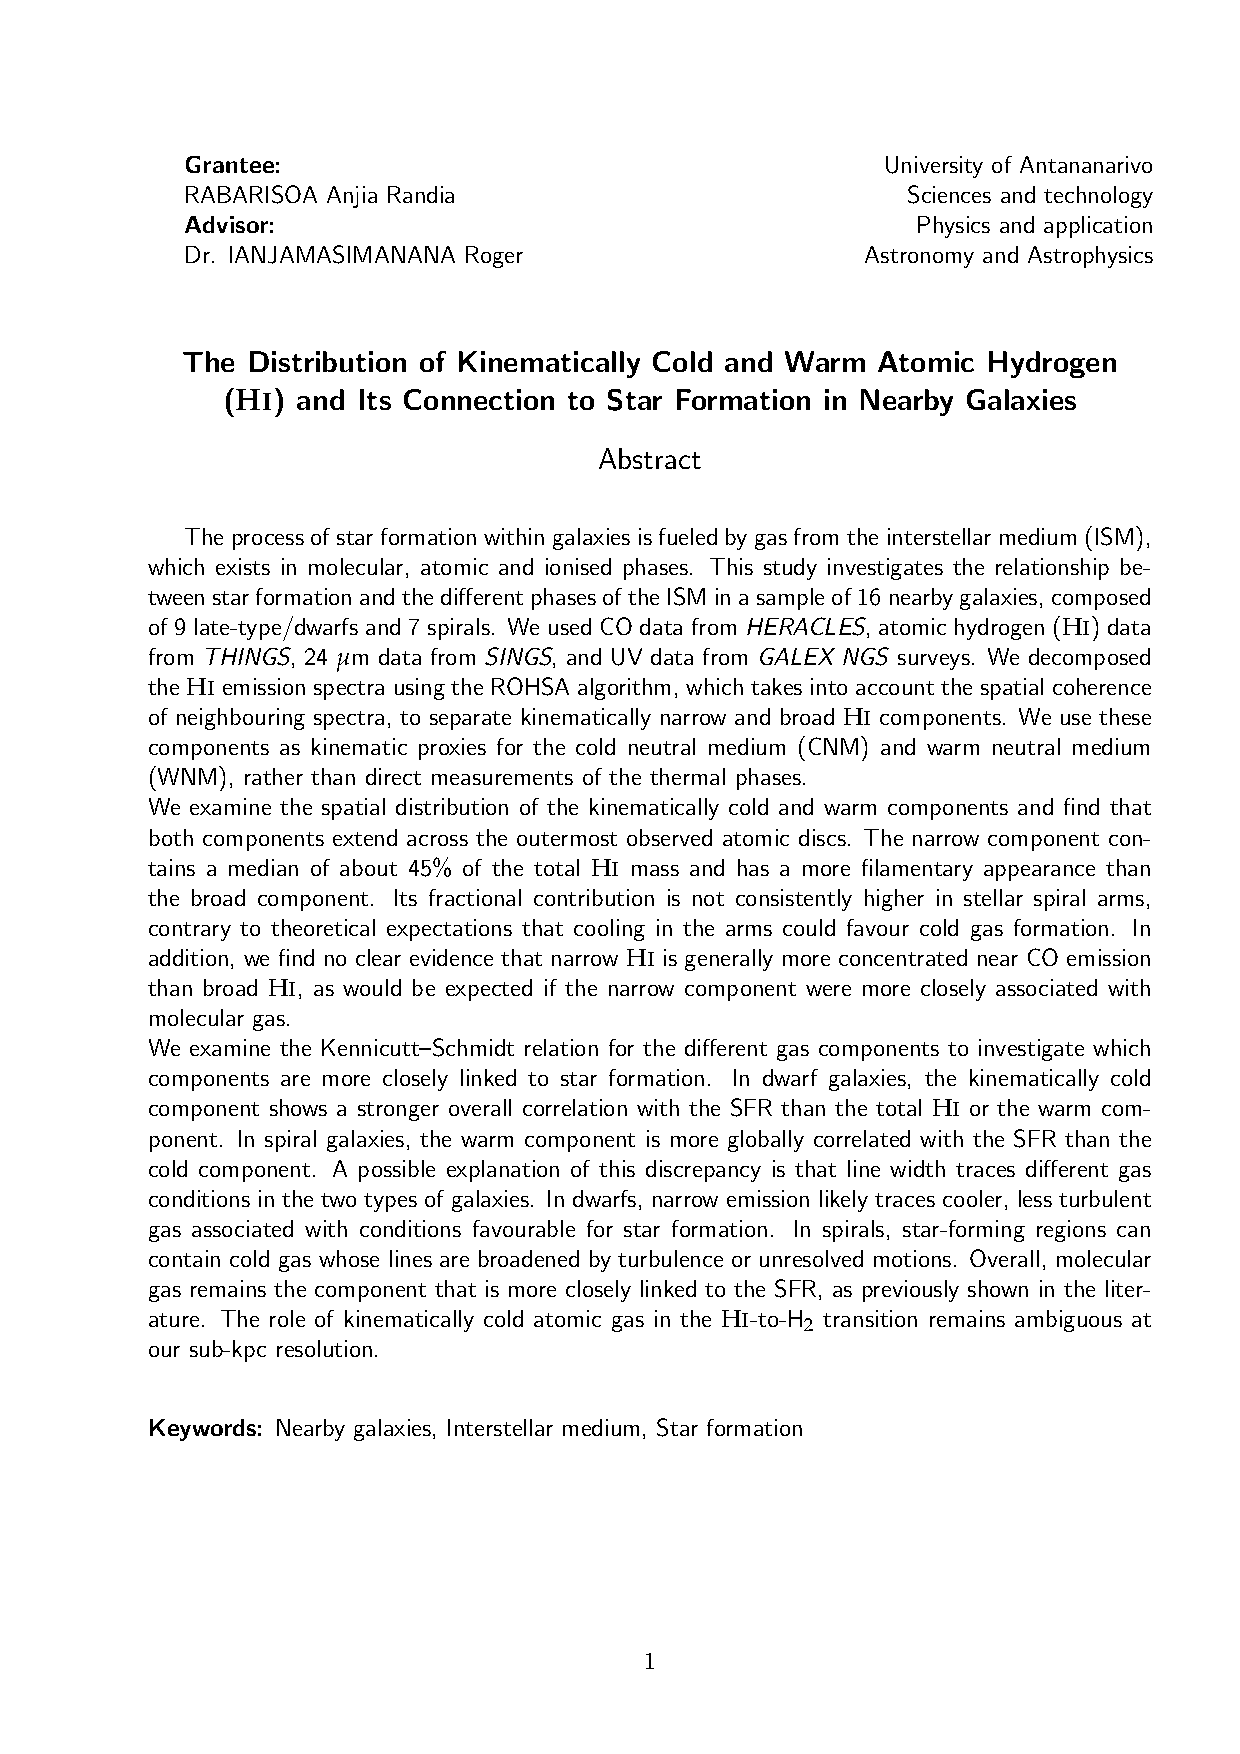
\includepdf[pages=-]{./Appendix/abstract_cover}
\end{document}
